%% abtex2-modelo-trabalho-academico.tex, v-1.9.6 laurocesar
%% Copyright 2012-2016 by abnTeX2 group at http://www.abntex.net.br/ 
%%
%% This work may be distributed and/or modified under the
%% conditions of the LaTeX Project Public License, either version 1.3
%% of this license or (at your option) any later version.
%% The latest version of this license is in
%%   http://www.latex-project.org/lppl.txt
%% and version 1.3 or later is part of all distributions of LaTeX
%% version 2005/12/01 or later.
%%
%% This work has the L PPL maintenance status `maintained'.
%% 
%% The Current Maintainer of this work is the abnTeX2 team, led
%% by Lauro César Araujo. Further information are available on 
%% http://www.abntex.net.br/
%%
%% This work consists of the files abntex2-modelo-trabalho-academico.tex,
%% abntex2-modelo-include-comandos and abntex2-modelo-references.bib
% ------------------------------------------------------------------------
% ------------------------------------------------------------------------
% abnTeX2: Modelo de Trabalho Academico (tese de doutorado, dissertacao de
% mestrado e trabalhos monograficos em geral) em conformidade com 
% ABNT NBR 14724:2011: Informacao e documentacao - Trabalhos academicos -
% Apresentacao
% ------------------------------------------------------------------------
% ------------------------------------------------------------------------
% Personalização para o modelo Udesc 2020 7. ed. revisada e modificada
% MANUAL_2020_09_07_1599489825065_12510.pdf
% Autor: Felipe Joel Zimann (felipezimann@hotmail.com)
% Data: 02/12/2020 v1.0
% Data: 13/02/2021 v1.0.1 alterado tamanho numeração da página para 10pt
% ------------------------------------------------------------------------
% ------------------------------------------------------------------------

\documentclass[
	12pt,					% tamanho da fonte
	openright,				% capítulos começam em pág ímpar (insere página vazia caso preciso)
	oneside,				% para impressão em recto e verso (twoside). Oposto a (oneside)
	a4paper,				% tamanho do papel. 
	chapter=TITLE,			% títulos de capítulos convertidos em letras maiúsculas
	section=TITLE,			% títulos de seções convertidos em letras maiúsculas
	sumario=abnt-6027-2012,
	english,				% idioma adicional para hifenização
	brazil,					% o último idioma é o principal do documento
	fleqn,					% equações alinhadas a esquerda (UDESC/CCT)+
	]{abntex2}

% ----------------------------------------------------------
% Pacotes básicos 
% ----------------------------------------------------------
\usepackage{amsmath}							% Pacote matemático
\usepackage{amssymb}							% Pacote matemático
\usepackage{amsfonts}							% Pacote matemático
%\usepackage{lmodern}							% Usa a fonte Latin Modern		
\usepackage{mathptmx} 							% Usa a fonte Times New Roman	 (UDESC/CCT)
\usepackage[T1]{fontenc}						% Selecao de codigos de fonte.
\usepackage[utf8]{inputenc}						% Codificacao do documento (conversão automática dos acentos)
\usepackage{lastpage}							% Usado pela Ficha catalográfica
\usepackage{indentfirst}						% Indenta o primeiro parágrafo de cada seção.
\usepackage[dvipsnames,table]{xcolor}			% Controle das cores
\usepackage{graphicx}							% Inclusão de gráficos
\usepackage{microtype} 							% para melhorias de justificação
\usepackage{lipsum}								% para geração de dummy text
\usepackage[brazilian,hyperpageref]{backref}	% Paginas com as citações na bibl
\usepackage[alf,abnt-emphasize=bf,abnt-full-initials=yes]{abntex2cite}					% Citações padrão ABNT
%\usepackage[num]{abntex2cite}					% Citações padrão ABNT numérica
\usepackage{adjustbox}							% Pacote de ajuste de boxes
\usepackage{subcaption}							% Inclusão de Subfiguras e sublegendas		
\usepackage{enumitem}							% Personalização de listas
\usepackage{siunitx}							% Grandezas e unidades
\usepackage[section]{placeins}					% Manter as figuras delimitadas na respectiva seção com a opção [section]
\usepackage{multirow}							% Multi colunas nas tabelas
\usepackage{array,tabularx} 					% Pacotes de tabelas
\usepackage{booktabs}							% Pacote de tabela profissonal
\usepackage{rotating}							% Rotacionar figuras e tabelas
\usepackage{xfrac}								% Fazer frações n/d em linha
\usepackage{bm}									% Negrito em modo matemático
\usepackage{xstring}							% Manipulação de strings
\usepackage{pgfplots}							% Pacote de Gráficos
\usepackage{tikz}								% Pacote de Figuras
\usepackage[american, cuteinductors,smartlabels, fulldiode, siunitx, americanvoltages, oldvoltagedirection, smartlabels]{circuitikz}						% Pacote de circuitos elétricos
\usepackage{chemformula}						% Pacote para fórmulas químicas
\usepackage{chngcntr}							% Pacte usado para deixar numeração de equações sequencial (UDESC/CCT)
\counterwithout{equation}{chapter}
% fonte: https://latex.org/forum/viewtopic.php?t=15392

% Comando para deixar numeração das equações contínua (1), (2), (3)... ao invés de organizar por capítulos (1.1)(1.2)... (2.1)(2.2)
%\renewcommand{\theequation}{\arabic{equation}}

%\numberwithin{equation}{section}


% Cabecalho cabeçalho somente com numeração de página 10pt
\makepagestyle{PagNumReduzida}
\makeevenhead{PagNumReduzida}{\ABNTEXfontereduzida\thepage}{}{}
\makeoddhead{PagNumReduzida}{}{}{\ABNTEXfontereduzida\thepage}
%fonte: https://github.com/abntex/abntex2/wiki/HowToCustomizarCabecalhoRodape
%fonte: Manual memoir seção 7.3 pg. 111 pdf http://linorg.usp.br/CTAN/macros/latex/contrib/memoir/memman.pdf 

% Personalização das opções das listas
\setlist[itemize]{leftmargin=\parindent}

% Citação online --- MODIFICAR ---
\newcommand{\citeshort}[1]{\citeauthoronline{#1}~(\citeyear{#1})}

\newcommand{\me}[1]{Elaborado pelo autor (#1).}

% Configuração do pgfplots
\pgfplotsset{compat=newest} %compat=1.14
\pgfplotsset{plot coordinates/math parser=false} 
\newlength\figureheight 
\newlength\figurewidth 

% Libraries do TiKz
\usetikzlibrary{quotes,angles,arrows}
\usetikzlibrary{through,calc,math}
\usetikzlibrary{graphs,backgrounds,fit}
\usetikzlibrary{shapes,positioning,patterns,shadows}
\usetikzlibrary{decorations.pathreplacing}
\usetikzlibrary{shapes.geometric}
\usetikzlibrary{arrows.meta}
\usetikzlibrary{external}

%\tikzexternalize[]
%\tikzexternalenable
%\tikzexternalize
%\tikzexternaldisable
%\tikzset{external/force remake}
%\tikzexternalize[shell escape=-enable-write18]

% Configurações do CircuiTiKz
\ctikzset{bipoles/thickness=1}
%\ctikzset{bipoles/length=1.2cm}
\ctikzset{monopoles/ground/width/.initial=.2}
\ctikzset{bipoles/resistor/height=0.25}
\ctikzset{bipoles/resistor/width=0.6}
\ctikzset{bipoles/capacitor/height=0.5}
\ctikzset{bipoles/capacitor/width=0.15}
\ctikzset{bipoles/generic/height=0.25}
\ctikzset{bipoles/generic/width=0.6}
%\ctikzset{bipoles/capacitor polar/length=0.5}
%\ctikzset{bipoles/diode/height=.375}
%\ctikzset{bipoles/diode/width=.3}
%\ctikzset{tripoles/thyristor/height=.8}
%\ctikzset{tripoles/thyristor/width=1}
\ctikzset{bipoles/vsourcesin/height=.5}
\ctikzset{bipoles/vsourcesin/width=.5}
\ctikzset{bipoles/cvsourceam/height=.6}
\ctikzset{bipoles/cvsourceam/width=.6}
%\ctikzset{tripoles/european controlled voltage source/width=.4}

\tikzstyle{every node}=[font=\footnotesize]
\tikzstyle{every path}=[line width=0.25pt,line cap=round,line join=round]
%\tikzstyle{every path}=[line cap=round,line join=round]


% Definição de cores MATLAB
\definecolor{matlab_blue}{rgb}	{         0,    0.4470,    0.7410}
\definecolor{matlab_orange}{rgb}{    0.8500,    0.3250,    0.0980}
\definecolor{matlab_yellow}{rgb}{    0.9290,    0.6940,    0.1250}
\definecolor{matlab_violet}{rgb}{    0.4940,    0.1840,    0.5560}
\definecolor{matlab_green}{rgb}	{	 0.4660,    0.6740,    0.1880}
\definecolor{matlab_lblue}{rgb}	{    0.3010,    0.7450,    0.9330}
\definecolor{matlab_red}{rgb}	{    0.6350,    0.0780,    0.1840}

% Personalização das legendas
\usepackage[format = plain, %hang
			justification = centering,
			labelsep = endash,
			singlelinecheck = false,
			skip = 6pt,
			listformat = simple]{caption}	

% Personalização das unidades
\sisetup{output-decimal-marker = {,}}
\sisetup{exponent-product = \cdot, output-product = \cdot}
\sisetup{tight-spacing=true}
\sisetup{group-digits = false}

% Personalizações de tipo de colunas de tabelas
\newcolumntype{L}[1]{>{\raggedright\let\newline\\\arraybackslash\hspace{0pt}}m{#1}}
\newcolumntype{C}[1]{>{\centering\let\newline\\\arraybackslash\hspace{0pt}}m{#1}}
\newcolumntype{R}[1]{>{\raggedleft\let\newline\\\arraybackslash\hspace{0pt}}m{#1}}

% Personalizações de cores da UDESC
\definecolor{CapaAmareloUDESC}{RGB}{243,186,83}		% Especializacao
\definecolor{CapaVerdeUDESC}{RGB}{0,112,52}			% Mestrado
\definecolor{CapaVermelhoUDESC}{RGB}{171,35,21}		% Doutorado
\definecolor{CapaAzulUDESC}{RGB}{38,54,118} 		% Pós-Doutorado

% CONFIGURAÇÕES DE PACOTES
% Configurações do pacote backref
% Usado sem a opção hyperpageref de backref
\renewcommand{\backrefpagesname}{Citado na(s) página(s):~}
% Texto padrão antes do número das páginas
\renewcommand{\backref}{}
% Define os textos da citação
\renewcommand*{\backrefalt}[4]{
	\ifcase #1 %
	Nenhuma citação no texto.%
	\or
	Citado na página #2.%
	\else
	Citado #1 vezes nas páginas #2.%
	\fi}%

% alterando o aspecto da cor azul
%\definecolor{blue}{RGB}{41,5,195}

% informações do PDF
\makeatletter
\hypersetup{
	%pagebackref=true,
	pdftitle={\@title}, 
	pdfauthor={\@author},
	pdfsubject={\imprimirpreambulo},
	pdfcreator={LaTeX with abnTeX2},
	pdfkeywords={abnt}{latex}{abntex}{abntex2}{trabalho academico}, 
	colorlinks=true,       		% false: boxed links; true: colored links
	linkcolor=black,          	% color of internal links
	citecolor=black,        	% color of links to bibliography
	filecolor=black,      		% color of file links
	urlcolor=black,
	bookmarksdepth=4
}
\makeatother


\makeatletter
\newcommand{\includetikz}[1]{%
	\tikzsetnextfilename{#1}%
	\input{#1.tex}%
}
\makeatother

% ---
% Possibilita criação de Quadros e Lista de quadros.
% Ver https://github.com/abntex/abntex2/issues/176
%
\newcommand{\quadroname}{Quadro}
\newcommand{\listofquadrosname}{Lista de quadros}

\newfloat[chapter]{quadro}{loq}{\quadroname}
\newlistof{listofquadros}{loq}{\listofquadrosname}
\newlistentry{quadro}{loq}{0}

% configurações para atender às regras da ABNT
\setfloatadjustment{quadro}{\centering}
\counterwithout{quadro}{chapter}
\renewcommand{\cftquadroname}{\quadroname\space} 
\renewcommand*{\cftquadroaftersnum}{\hfill--\hfill}

\setfloatlocations{quadro}{hbtp} % Ver https://github.com/abntex/abntex2/issues/176
% ---


% Espaçamento depois do título
\setlength{\afterchapskip}{0.7\baselineskip}
% O tamanho do parágrafo é dado por:
\setlength{\parindent}{1.25cm}
% Controle do espaçamento entre um parágrafo e outro:
\setlength{\parskip}{0.0cm}  % tente também \onelineskip
%\SingleSpacing % Espaçamento simples 
\OnehalfSpacing % Espaçamento 1,5 (UDESC/CCT)
%\DoubleSpacing	% Espaçamento duplo

% ---
% Margens - NBR 14724/2011 - 5.1 Formato
% ---
\setlrmarginsandblock{3cm}{2cm}{*}
\setulmarginsandblock{3cm}{2cm}{*}
\checkandfixthelayout[fixed]
% ---


% To use externalize consider
%https://tex.stackexchange.com/questions/182783/tikzexternalize-not-compatible-with-miktex-2-9-abntex2-package
%Lauro Cesar digged into the problem until he came with a solution for me to test. And it Works!
%
%According to this link:
%
%The package calc changed the commands \setcounter and friends to be fragile. So you have to make them robust. The example below uses etoolbox with \robustify:
%
\usepackage{etoolbox}
\robustify\setcounter
\robustify\addtocounter
\robustify\setlength
\robustify\addtolength


%% How to silence memoir class warning against the use of caption package?
%% https://tex.stackexchange.com/questions/391993/how-to-silence-memoir-class-warning-against-the-use-of-caption-package
%\usepackage{silence}
%\WarningFilter*{memoir}{You are using the caption package with the memoir class}
%\WarningFilter*{Class memoir Warning}{You are using the caption package with the memoir class}

% --------------------------------------------------------
% INICIO DAS CUSTOMIZACOES PARA A UDESC
% --------------------------------------------------------

% --------------------------------------------------------
% Fontes padroes de part, chapter, section, subsection e subsubsection
% --------------------------------------------------------
% --- Chapter ---
\renewcommand{\ABNTEXchapterfont}{\fontseries{b}} %\bfseries
\renewcommand{\ABNTEXchapterfontsize}{\normalsize}
% --- Part ---
\renewcommand{\ABNTEXpartfont}{\ABNTEXchapterfont}
\renewcommand{\ABNTEXpartfontsize}{\LARGE}
% --- Section ---
\renewcommand{\ABNTEXsectionfont}{\normalfont}
\renewcommand{\ABNTEXsectionfontsize}{\normalsize}
% --- SubSection ---
\renewcommand{\ABNTEXsubsectionfont}{\fontseries{b}} %\bfseries
\renewcommand{\ABNTEXsubsectionfontsize}{\normalsize}
% --- SubSubSection ---
\renewcommand{\ABNTEXsubsubsectionfont}{\itshape}
\renewcommand{\ABNTEXsubsubsectionfontsize}{\normalsize}

\renewcommand{\ABNTEXsubsubsubsectionfont}{\normalfont}
\renewcommand{\ABNTEXsubsubsubsectionfontsize}{\normalsize}
% ---

% --------------------------------------------------------
% Fontes das entradas do sumario
% --------------------------------------------------------

\renewcommand{\cftpartfont}{\ABNTEXpartfont\selectfont}
\renewcommand{\cftpartpagefont}{\normalsize\selectfont}

\renewcommand{\cftchapterfont}{\ABNTEXchapterfont\selectfont}
\renewcommand{\cftchapterpagefont}{\normalsize\selectfont}

\renewcommand{\cftsectionfont}{\ABNTEXsectionfont\selectfont}
\renewcommand{\cftsectionpagefont}{\normalsize\selectfont}

\renewcommand{\cftsubsectionfont}{\ABNTEXsubsectionfont\selectfont}
\renewcommand{\cftsubsectionpagefont}{\normalsize\selectfont}

\renewcommand{\cftsubsubsectionfont}{\normalfont\itshape\selectfont}
\renewcommand{\cftsubsubsectionpagefont}{\normalsize\selectfont}

\renewcommand{\cftparagraphfont}{\normalfont\selectfont}
\renewcommand{\cftparagraphpagefont}{\normalsize\selectfont}

% --------------------------------------------------------
% Usando os pacotes hyperref, uppercase... 
% Para deixar a section do toc uppercase precisa de:
% --------------------------------------------------------
\usepackage{textcase}

\makeatletter

\let\oldcontentsline\contentsline
\def\contentsline#1#2{%
	\expandafter\ifx\csname l@#1\endcsname\l@section
	\expandafter\@firstoftwo
	\else
	\expandafter\@secondoftwo
	\fi
	{%
		\oldcontentsline{#1}{\MakeTextUppercase{#2}}%
	}{%
		\oldcontentsline{#1}{#2}%
	}%
}
\makeatother

% --------------------------------------------------------
% Renomenando as entradas de APÊNDICES E ANEXOS
% --------------------------------------------------------

\renewcommand{\apendicesname}{AP\^ENDICES}
\renewcommand{\anexosname}{ANEXOS}


% Manipulação de Strings
%\RequirePackage{xstring}

% Comando para inverter sobrenome e nome
\newcommand{\invertname}[1]{%
	\StrBehind{#1}{{}}, \StrBefore{#1}{{}}%
}%


% --------------------------------------------------------
% Alterando os estilos de Caption e Fonte
% --------------------------------------------------------
\makeatletter
% Define o comando \fonte que respeita as configurações de caption do memoir ou do caption
\renewcommand{\fonte}[2][\fontename]{%
	\M@gettitle{#2}%
	\memlegendinfo{#2}%
	\par
	\begingroup
	\@parboxrestore
	\if@minipage
	\@setminipage
	\fi
	\ABNTEXfontereduzida
	\configureseparator
	\captiondelim{\ABNTEXcaptionfontedelim}
	\@makecaption{#1}{\ignorespaces #2}\par
	\endgroup}


\captionstyle[\raggedright]{\raggedright}

\makeatother

\setlength{\cftbeforechapterskip}{0pt plus 0pt}
\renewcommand*{\insertchapterspace}{}

\newlength{\mylen}	% New length to use with spacing
\setlength{\mylen}{1pt}

\setlength{\cftbeforechapterskip}{\mylen}
\setlength{\cftbeforesectionskip}{\mylen}
\setlength{\cftbeforesubsectionskip}{\mylen}
\setlength{\cftbeforesubsubsectionskip}{\mylen}
\setlength{\cftbeforesubsubsubsectionskip}{\mylen}


% ---
% Ajuste das listas de abreviaturas e siglas ; e símbolos [Personalizada para UDESC com espaçamento 1,5]
% ---

% ---
% Redefinição da Lista de abreviaturas e siglas [Personalizada para UDESC com espaçamento 1,5]
\renewenvironment{siglas}{%
	\pretextualchapter{\listadesiglasname}
	\begin{symbols} 
		\setlength{\itemsep}{0pt}	% Ajuste para Espaçamento 1,5 (UDESC/CCT)
	}{% 
	\end{symbols}
	\cleardoublepage
}
% ---

% ---
% Redefinição da Lista de símbolos [Personalizada para UDESC com espaçamento 1,5]
\renewenvironment{simbolos}{%
	\pretextualchapter{\listadesimbolosname}
	\begin{symbols}
		\setlength{\itemsep}{0pt}	% Ajuste para Espaçamento 1,5 (UDESC/CCT)
	}{%
	\end{symbols}
	\cleardoublepage
}
% ---





% ---
% FIM DAS CUSTOMIZACOES PARA A  Universidade do Estado de Santa Catarina - UDESC/CCT
% ---





	% Incliu pacotes básicos 

% -----------------------------------------------------------------
% Você pode adicionar seus pacotes a partir desta linha;
% -----------------------------------------------------------------

%\usepackage[showframe,pass]{geometry}
%\usepackage[11,12]{pagesel}

% -----------------------------------------------------------------
% Informações de dados para CAPA e FOLHA DE ROSTO
% -----------------------------------------------------------------
\titulo{Estudo e comparação de algoritmos para encaminhamento de fluxos em redes definidas por software}%

\autor{Devair Dener {}Darolt}%
\orientador{Guilherme Koslovski}%
%\coorientador{Nome do coorientador{} Sobrenome}%

% ATENÇÃO: O símbolo {} indica o sobrenome para a ficha catalográfica.
% Exemplo: Sherlock Holmes {}da Silva para sobrenomes compostos;
% Exemplo: Arnold Alois {}Schwarzenegger para sobrenome simples.

\instituicao{Universidade do Estado de Santa Catarina, Centro de Ciências Tecnológicas, Bacharelado em ciência da computação}%

%\tipotrabalho{Tese (Doutorado)}
\tipotrabalho{Monografia (Graduação)}

%\preambulo{Tese apresentada ao Programa de Pós--Graduação em Engenharia Elétrica do Centro de Ciências Tecnológicas da Universidade do Estado de Santa Catarina, como requisito parcial para a obtenção do grau de Doutor em Engenharia Elétrica.}

\preambulo{Monografia apresentada a disciplina de Trabalho de Conclusão de Curso II, do curso de ciência da computação do CCT/UDESC, como requisito para obtenção do título de bacharel em ciência da computação.}

\local{Joinville}%

\data{\the\year}%
% ---

% compila o indice
\makeindex

% -----------------------------------------------------------------
% Início do documento
% -----------------------------------------------------------------
\begin{document}

\selectlanguage{brazil}
\frenchspacing  % Retira espaço extra obsoleto entre as frases.

% -----------------------------------------------------------------
% ELEMENTOS PRÉ-TEXTUAIS
% -----------------------------------------------------------------
\pretextual

% Você pode comentar os elementos que não deseja em seu trabalho;

% A capa pode ser escolhida dentro do arquivo Capa.tex (TCC, Master, Doc, ...)
% ---
% Capa
% ---


% --------------------------------------------------------
% Capa Padrão
% --------------------------------------------------------
\renewcommand{\imprimircapa}{%
	\begin{capa}%
		\center

		{\fontseries{b}\selectfont\MakeTextUppercase{UNIVERSIDADE DO ESTADO DE SANTA CATARINA -- UDESC}}
		
		{\fontseries{b}\selectfont\MakeTextUppercase{CENTRO DE CIÊNCIAS TECNOLÓGICAS -- CCT  }}
		
		{\fontseries{b}\selectfont\MakeTextUppercase{BACHARELADO EM CIÊNCIA DA COMPUTAÇÃO -- BCC }}
		\vfill
		
		{\fontseries{b}\selectfont\MakeTextUppercase{\normalsize\imprimirautor}}
		
		\vfill
		\begin{center}
			{\fontseries{b}\selectfont\MakeTextUppercase{\imprimirtitulo}}
		\end{center}
		\vfill
		
		\vfill
		
		{\fontseries{b}\selectfont\MakeTextUppercase{\imprimirlocal}}
		\par
		{\fontseries{b}\selectfont \imprimirdata}
		\vspace*{1cm}
	\end{capa}
}



\imprimircapa				% Capa padrão

					% Elemento Obrigatório
% ---
% Folha de rosto
% ---








% --------------------------------------------------------
% folha de rosto 
% --------------------------------------------------------

\makeatletter

\renewcommand{\folhaderostocontent}{
	\begin{center}
		
		{\fontseries{b}\selectfont\MakeTextUppercase{\imprimirautor}}
		
		\vfill
		
		\begin{center}
			{\fontseries{b}\selectfont\MakeTextUppercase{\imprimirtitulo}}
		\end{center}
	
		\vspace*{1.5cm}

		\abntex@ifnotempty{\imprimirpreambulo}{%
			\hspace{.45\textwidth}
			{\begin{minipage}{.5\textwidth}
					\SingleSpacing
					\imprimirpreambulo\par
					\vspace*{4pt}
					{\imprimirorientadorRotulo~\imprimirorientador\par}
					\abntex@ifnotempty{\imprimircoorientador}{%
						{\imprimircoorientadorRotulo~\imprimircoorientador}%
					}%
			\end{minipage}}%
		}%
	
		
		\vfill
		
	{\fontseries{b}\selectfont\MakeTextUppercase{\imprimirlocal}}
	\par
	{\fontseries{b}\selectfont \imprimirdata}
	\vspace*{1cm}
	\end{center}
}


% (o * indica que haverá a ficha bibliográfica)
% ---
\imprimirfolhaderosto*
% ---


			% Elemento Obrigatório
% Caso não utilize a Ficha Catalográfica entre na folha de rosto e retire o * de dentro do arquivo FolhadeRosto
%
% ---
% Inserir a ficha bibliografica
% ---

% Isto é um exemplo de Ficha Catalográfica, ou ``Dados internacionais de
% catalogação-na-publicação''. Você pode utilizar este modelo como referência. 
% Porém, provavelmente a biblioteca da sua universidade lhe fornecerá um PDF
% com a ficha catalográfica definitiva após a defesa do trabalho. Quando estiver
% com o documento, salve-o como PDF no diretório do seu projeto e substitua todo
% o conteúdo de implementação deste arquivo pelo comando abaixo:



% \begin{fichacatalografica}
%     \includepdf{fig_ficha_catalografica.pdf}
% \end{fichacatalografica}


%	\setlength{\parindent}{0cm}
%	\setlength{\parskip}{0pt}
\begin{fichacatalografica}
	%\sffamily
	%\rmfamily
	\ttfamily \hbadness=10000
	\vspace*{\fill}					% Posição vertical
	\begin{center}					% Minipage Centralizado
	Para gerar a ficha catalográfica de teses e \\ 
	dissertações acessar o link:  \\
	https://www.udesc.br/bu/manuais/ficha
	
	\vspace*{8pt}
	
%	\begin{minipage}[c]{8cm}
%	\centering \sffamily
%	 Ficha catalográfica elaborada pelo(a) autor(a), com auxílio do programa de geração automática da Biblioteca Setorial do CCT/UDESC
%	\end{minipage}
	\fbox{\begin{minipage}[c]{12.5cm}		% Largura
	\flushright
	{\begin{minipage}[c]{10.5cm}		% Largura
	\vspace{1.25cm}
	%\footnotesize
	\setlength{\parindent}{1.5em}
	\noindent \invertname{\imprimirautor} \par
	\imprimirtitulo{ }/{ }\imprimirautor. -- \imprimirlocal, \imprimirdata .\par
	\pageref{LastPage} p. : il. ; 30 cm.\par
	\vspace{1.5em}
	\imprimirorientadorRotulo~\imprimirorientador.\par
	\imprimircoorientadorRotulo~\imprimircoorientador.\par
	\imprimirtipotrabalho~--~\imprimirinstituicao, \imprimirlocal, \imprimirdata.\par
	\vspace{1.5em}
		1. Engenharia de Tráfego.
		2. Floodlight.
		3. OpenFlow.
 		4. Mininet.
		5. SDN.
		I. \invertname{\imprimirorientador}.
		II. \invertname{\imprimircoorientador}.
		III. \imprimirinstituicao.
		IV. Título. %
	\vspace{1.25cm}	%		
	\end{minipage}%
	}% 
	\end{minipage}}%
	
	\vspace*{0.5cm}
	
	\end{center}
\end{fichacatalografica}


%\begin{fichacatalografica}
%	\sffamily
%	\vspace*{\fill}					% Posição vertical
%	\begin{center}					% Minipage Centralizado
%	\fbox{\begin{minipage}[c][8cm]{13.5cm}		% Largura
%	\small
%	\imprimirautor
%	%Sobrenome, Nome do autor
%	
%	\hspace{0.5cm} \imprimirtitulo  / \imprimirautor. --
%	\imprimirlocal, \imprimirdata-
%	
%	\hspace{0.5cm} \pageref{LastPage} p. : il. (algumas color.) ; 30 cm.\\
%	
%	\hspace{0.5cm} \imprimirorientadorRotulo~\imprimirorientador\\
%	
%	\hspace{0.5cm}
%	\parbox[t]{\textwidth}{\imprimirtipotrabalho~--~\imprimirinstituicao,
%	\imprimirdata.}\\
%	
%	\hspace{0.5cm}
%		1. Palavra-chave1.
%		2. Palavra-chave2.
%		3. Palavra-chave3.
% 		4. Palavra-chave4.
%		5. Palavra-chave5.
%		I. Orientador.
%		II. Universidade xxx.
%		III. Faculdade de xxx.
%		IV. Título 			
%	\end{minipage}}
%	\end{center}
%\end{fichacatalografica}
% ---

	% Elemento Obrigatório (Verso da Folha)
%
% ---
% Inserir errata
% ---
\begin{errata}
Elemento opcional. 

Exemplo:

\vspace{\onelineskip}

SOBRENOME, Prenome do Autor. Título de obra: subtítulo (se houver). Ano de depósito. Tipo do trabalho (grau e curso) - Vinculação acadêmica, local de apresentação/defesa, data.

\begin{table}[htb]
\center
\begin{tabular}{|p{2.4cm}|p{2cm}|p{3cm}|p{3cm}|}
  \hline
   \textbf{Folha} & \textbf{Linha}  & \textbf{Onde se lê}  & \textbf{Leia-se}  \\
    \hline
    1 & 10 & auto-conclavo & autoconclavo\\
   \hline
\end{tabular}
\end{table}

\end{errata}
% ---				% Elemento Opcional

% ---
% Inserir folha de aprovação
% ---

% Isto é um exemplo de Folha de aprovação, elemento obrigatório da NBR
% 14724/2011 (seção 4.2.1.3). Você pode utilizar este modelo até a aprovação
% do trabalho. Após isso, substitua todo o conteúdo deste arquivo por uma
% imagem da página assinada pela banca com o comando abaixo:
%
% \includepdf{folhadeaprovacao_final.pdf}
%
\begin{folhadeaprovacao}



	\begin{center}
		{\fontseries{b}\selectfont\MakeTextUppercase{\normalsize\imprimirautor}}
	\end{center}
    \vfill
    
	\vfill
	\begin{center}
		{\fontseries{b}\selectfont\MakeTextUppercase{\imprimirtitulo}}
	\end{center}
	\vfill

    
\abntex@ifnotempty{\imprimirpreambulo}{%
	\hspace{.45\textwidth}
	{\begin{minipage}{.5\textwidth}
			\SingleSpacing
			\imprimirpreambulo\par
			\vspace*{4pt}
			{\imprimirorientadorRotulo~\imprimirorientador\par}
			\abntex@ifnotempty{\imprimircoorientador}{%
				{\imprimircoorientadorRotulo~\imprimircoorientador}%
			}%
	\end{minipage}}%
}%


\vfill
        
	 \begin{center}
	 	
    	{\fontseries{b}\selectfont BANCA EXAMINADORA: }
    	\vspace*{1.75cm}
    
        \assinatura{\textbf{} }
		Guilherme Piêgas Koslovski - Doutor (Orientador)\par
		CCT/UDESC
	 \end{center}
	
    %{Membros:} 
    
	\begin{center}
		\vspace*{1.25cm}
		\assinatura{\textbf{} }
		Charles Christian Miers - Doutor \par
		CCT/UDESC
		
		\vspace*{1.25cm}
		\assinatura{\textbf{} }
		Maurício Aronne Pillon - Doutor \par
		CCT/UDESC
		
		
	\end{center}
    
    \vspace*{\fill}  
    \begin{center}
    {\imprimirlocal, 10 de Agosto de \imprimirdata}
	\end{center}
    \vspace*{0.25cm}  
\end{folhadeaprovacao}
% ---




%\textbf{	{Orientador: \vspace{-16pt} }
	%\assinatura{\textbf{Prof. \imprimirorientador , Dr.} \\ Univ. XXX} 
	%{Coorientador: \vspace{-16pt}}   
	%\assinatura{\textbf{Prof. \imprimircoorientador , Dr.} \\ Univ. XXX}
	
	%{Membros: \vspace{-16pt} } 
	
	% --- Exemplo de assinaturas em sequência ---       
	%\setlength{\ABNTEXsignwidth}{8.5cm}
	
	%\assinatura{\textbf{Prof. Professor, Dr.} \\ Univ. XXX}
	%\assinatura{\textbf{Prof. Professor, Dr.} \\ Univ. XXX}
	%\assinatura{\textbf{Prof. Professor, Dr.} \\ Univ. XXX}
	
	% --- Exemplo de assinaturas lado a lado ---
	%\setlength{\ABNTEXsignwidth}{7.5cm}
%
    %\noindent\hfill\assinatura*{\textbf{Prof. Professor, Dr.} \\ Univ. XXX}%
	    %\hfill%
	    %\assinatura*{\textbf{Prof. Professor, Dr.} \\ Univ. XXX}%
	    %\hfill
	    
	   % \noindent\hfill\assinatura*{\textbf{Prof. Professor, Dr.} \\ Univ. XXX}%
	  %  \hfill%
	 %   \assinatura*{\textbf{Prof. Professor, Dr.} \\ Univ. XXX}%
	%    \hfill}		% Elemento Obrigatório
% ---
% Dedicatória
% ---
\begin{dedicatoria}
   \vspace*{\fill}
%   \begin{flushright}
%   \noindent
%	Este trabalho é dedicado às crianças adultas que,\\
%	quando pequenas, sonharam em se tornar cientistas. 
%   \end{flushright}

{%
	\noindent\hspace{.5\textwidth}
	{\begin{minipage}{.5\textwidth}
			\begin{flushleft}
				Aos meus pais, amigos e professores da Universidade do Estado de Santa Catarina, pela inspiração de sempre!
			\end{flushleft}
	\end{minipage}}%
\vspace*{3cm}
}%

\end{dedicatoria}
% ---
			% Elemento Opcional
% ---
% Agradecimentos
% ---
\begin{agradecimentos}
Agradeço ao meu orientador Guilherme P. Koslovski por aceitar dar continuidade ao meu trabalho que já estava um tempo no fundo da gaveta.

A todos os meus professores do curso de Ciência da Computação da Universidade do Estado de Santa Catarina – Udesc pela qualidade técnica e esforço de cada um em transmitir seus conhecimentos, incentivando a buscar melhores resultados sempre.

Aos meus pais que estiveram sempre ao lado apoiando ao longo de toda a minha vida. Sou grato a minha família por todo esse apoio, não teria conseguido sem.

Deixo um agradecimento especial ao meu orientador pela dedicação do seu tempo a todos os meus projetos de pesquisas, nos quais pude aprender diversos tópicos interessantes, foram tempos memoráveis. Quero agradecer a Deus por sempre ajudar a superar os desafios, evoluir e buscar a verdade em todas as situações.

\end{agradecimentos}
% ---		% Elemento Opcional
%% ---
% Epígrafe
% ---
\begin{epigrafe}
    \vspace*{\fill}
%	\begin{flushright}
%		\textit{``Eu não falhei, encontrei 10 mil soluções que não davam certo.'' (EDISON, [19--])}
%	\end{flushright}
{%
	\noindent\hspace{.5\textwidth}
	{\begin{minipage}{.5\textwidth}
		\begin{flushright}
			``Eu não falhei, encontrei 10 mil soluções que não davam certo.'' (EDISON, [19--])
		\end{flushright}
	\end{minipage}}%
	\vspace*{3cm}
}%
\end{epigrafe}
% ---				% Elemento Opcional
% ---
% RESUMOS
% ---

% resumo em português
\setlength{\absparsep}{18pt} % ajusta o espaçamento dos parágrafos do resumo
\begin{resumo}
O paradigma de Redes Definidas por Software (SDN) foi recentemente difundido como uma das possibilidades para sobrepor a inflexibilidade dos recursos de comunicação, sobretudo da Internet.
Este paradigma, iniciado como um experimento acadêmico, vem sendo utilizado em cenários industriais (\textit{e.g.,} provedores de nuvens computacionais, provedores de conteúdo) pela facilidade de gerenciamento e implantação de inovações. 
A verticalização existente em redes convencionais limitou o desenvolvimento de protocolos e propostas arquiteturais durante décadas.
Em suma, SDN ultrapassou essa limitação através da separação dos planos de controle e dados nos dispositivos de comunicação.
O gerenciamento do plano de controle fica a cargo de componentes conectados à infraestrutura (controladores) que atuam sobre os dispositivos de encaminhamento através de abstrações.
Esse cenário flexível, permite a definição de novas políticas de controle e encaminhamento de fluxos por parte do administrador, implementadas diretamente no controlador. 
O alvo do presente trabalho é realizar um estudo comparativo entre políticas de encaminhamento de fluxos em SDN. Entre diversas estratégias existentes foram selecionadas 4 das mais comuns utilizadas. A primeira é a política de \textit{round-robin} (RR), que usa a estratégia de fila circular para alternar entre os múltiplos caminhos existentes. A segunda política é a do Caminho Mais Curto Reativo (CMCR), na qual, o controlador escolhe a cada salto o próximo comutador a ser enviado, de modo a utilizar o caminho de menor quantidade de saltos. A terceira política utilizada foi o Caminho Mais Curto Proativo  (CMCP) que implementa a lógica de menor quantidade de saltos, porém configurando todos os comutadores de uma única vez. Por último, a política de Caminho de Menor Tráfego (CMT) permite o controlador utiliza as informações de portas dos comutadores para encontrar o caminho com menor largura de banda utilizada. O cenário SDN será realizado com o emulador \textit{Mininet} enquanto os algoritmos de encaminhamento serão implementados no controlador \textit{Floodlight} e estudados com análise do desempenho da ferramenta \textit{Numerical Aerodynamic Simulation} (NAS).

 \textbf{Palavras-chave}: Engenharia de Tráfego, Floodlight, OpenFlow, Mininet, SDN.
\end{resumo}
				% Elemento Obrigatório
% ---
% Abstract
% ---

% resumo em inglês
\begin{resumo}[Abstract]
 \begin{otherlanguage*}{english}

The Software Defined Networks (SDN)  paradigm has recently been widespread as one of the possibilities to overcome the inflexibility of communication resources, especially the Internet. This paradigm, started as an academic experiment, has been used in industrial scenarios (\textit{e.g.}, cloud computing providers, content providers) due to the ease of managing and implementing innovations. The verticalization that exists in conventional networks has limited the development of protocols and architectural proposals for decades. SDN has overcome this limitation by separating control and data planes in communication devices. 
The control plane is managed by components connected to the infrastructure (controllers) that act on the forwarding devices through abstractions. This flexible scenario allows the definition of new control and flow forwarding policies by the administrator, implemented directly in the controller. 
The aim of this work is to carry out a comparative study between flow forwarding policies in SDN. Among several existing strategies, 4 of the most commonly used were selected. The first is the Round-Robin policy, which uses the circular queuing strategy to switch between existing multiple paths. 
The second policy is the shortest reactive path, in which the controller chooses at each hop the next switch to be sent, in order to use the path with the least number of hops. 
The third policy used was the proactive shortest path, in which the controller selects the path with the least amount of hops, but configuring all switches that belong to the path. 
Finally, the least traffic policy, which allows the controller to use the switch port information to find the path with the least bandwidth used. The SDN scenario will be performed with the Mininet emulator and the forwarding algorithms will be implemented in the Floodlight controller and analyzed through the performance of the Numerical Aerodynamic Simulation~(NAS) tools.

   \textbf{Keywords}: Floodlight, OpenFlow, Mininet, SDN, Traffic Engineering.
 \end{otherlanguage*}
\end{resumo}
				% Elemento Obrigatório
%\listofabbreviations{Lista de Abreviaturas}
\begin{acronym}
	\acro{API}[API]{Interface de Programação de Aplicações}
    \acro{ARP}[ARP]{\textit{Address Resolution Protocol}}
    \acro{ASIC}[ASIC]{\textit{Application-Specific Integrated Circuits}}
    \acro{AWMR}[AWMR]{\textit{Adaptive Worst-fit Multipath Routing}}
    \acro{BT}[BT]{\textit{Block-Tridiagonal}}
    \acro{BW}[BW]{\textit{Bandwidth}}
    \acro{CG}[CG]{\textit{Conjugate gradient}}
    \acro{CPU}[CPU]{Unidade Central de Processamento}
    \acro{DRAM}[DRAM]{Memória de Acesso Randômico Dinâmica}
    \acro{ECMP}[ECMP]{\textit{Equal-Cost Multi-Path}}
    \acro{EP}[EP]{\textit{Embarrassingly parallel}}
    \acro{FIFO}[FIFO]{ \textit{First In, First Out}}
    \acro{IP}[IP]{\textit{Internet Protocol}}
    \acro{IS}[IS]{\textit{Integer sort}}
    \acro{LU}[LU]{\textit{LU solver}}
    \acro{MAC}[MAC]{\textit{Media Access Control}}
    \acro{MG}[MG]{\textit{Multigrid}}
    \acro{MPI}[MPI]{\textit{Message Passing Interface}}
    \acro{MPTCP}[MPTCP]{\textit{Multipath TCP}}
    \acro{NAS}[NAS]{\textit{Numerical Aerodynamic Simulation}}
    \acro{NFV}[NFV]{\textit{Network Functions Virtualization}}
    \acro{NOS}[NOS]{\textit{Network Operation System}}
    \acro{OFRHM}[OFRHM]{\textit{OpenFlow Random Host Mutation}}
    \acro{ONF}[ONF]{\textit{Open Network Foundation}}
    \acro{OSPF}[OSPF]{\textit{Open Shortest Path First}}
    \acro{PF}[PF]{\textit{Proative Forwarding}}
    \acro{PSPacer/HT}[PSPacer/HT]{\textit{Precise Software Pacer/High-resolution Timer}}
    \acro{QoS}[QoS]{\textit{Quality of Service}}
    \acro{REST}[REST]{\textit{REpresentational State Transfer}}
    \acro{RF}[RF]{\textit{Reative Forwarding}}
	\acro{RR}[RR]{\textit{Round-Robin}}
	\acro{SDN}[SDN]{\textit{Software-Defined Networking}}
    \acro{SLA}[SLA]{\textit{Service Level Agreement}}
    \acro{SP}[SP]{\textit{Solution Pentadiagonal}}
    \acro{SSH}[SSH]{\textit{Secure Shell Protocol}}
    \acro{SSL}[SSL]{\textit{Secure Socket Layer}}
    \acro{TCAM}[TCAM]{\textit{Ternary Content- Addressable Memory})}
    \acro{TCP}[TCP]{\textit{Transmission Control Protocol}}
	\acro{TLS}[TLS]{\textit{Transport Layer Security}}
    \acro{URL}[URL]{\textit{Uniform Resource Identifier}}
    \acro{VLAN}[VLAN]{\textit{Virtual Local Area Network}}
    
    
\end{acronym}

% Defining: \acro{acronym}[short name]{full name}
% Usaging:
% \ac{acronym}     -- writes the full name followed by the acronym in brackets; later calls will write only the acronym
% \acf{acronym}     -- writes the full name followed by the acronym in brackets
% \acs{acronym}     -- writes the short name only
% \acl{acronym}     -- writes the full name only
% Use p at the end of previous commands for plural form (e.g., \acp for the plural form of \ac)
% \acresetall        -- reset usage of all acronyms (i.e., \ac will print full name again)
% \acused                -- mark the acronym as used

% ---
% inserir lista de ilustrações
% ---
\pdfbookmark[0]{\listfigurename}{lof}
\listoffigures*
\cleardoublepage
% ---

% ---
% inserir lista de quadros
% ---
%\pdfbookmark[0]{\listofquadrosname}{loq}
%\listofquadros*
%\cleardoublepage
% ---


% ---
% inserir lista de tabelas
% ---
\pdfbookmark[0]{\listtablename}{lot}
\listoftables*
\cleardoublepage
% ---

% ---
% inserir lista de abreviaturas e siglas
% ---
\begin{siglas}
    
    \item[ACL] \textit{Access Control List}
	\item[API] Interface de Programação de Aplicações
	\item[ARP] \textit{Address Resolution Protocol}
	\item[ASIC] \textit{Application-Specific Integrated Circuits}
	\item[BT]{\textit{Block-Tridiagonal}}
	\item[CG]{\textit{Conjugate gradient}}
	\item[CMCP]{Caminho Mais Curto Proativo}
	\item[CMCR]{Caminho Mais Curto Reativo}
	\item[CMT]{Caminho de Menor Tráfego}
	\item[CPU]{Unidade Central de Processamento}
	\item[DRAM]{Memória de Acesso Randômico Dinâmica}
	\item[EP]{\textit{Embarrassingly parallel}}
	\item[FIFO]{ \textit{First In, First Out}}
	\item[IIoT]{\textit{Industrial Internet of Things}}
	\item[IP]{\textit{Internet Protocol}}
	\item[IS]{\textit{Integer Sort}}
	\item[LU]{\textit{Lower Upper}}
	\item[MAC]{\textit{Media Access Control}}
	\item[MG]{\textit{Multigrid}}
	\item[MPI]{\textit{Message Passing Interface}}
	\item[NAS]{\textit{Numerical Aerodynamic Simulation}}
	\item[NASA]{\textit{National Aeronautics and Space Administration}}
	\item[NFV]{\textit{Network Functions Virtualization}}
	\item[NOS]{\textit{Network Operation System}}
	\item[NTT]{\textit{Nippon Telegraph and Telephone}}
	\item[OFRHM]{\textit{OpenFlow Random Host Mutation}}
	\item[ONF]{\textit{Open Network Foundation}}
	\item[QoS]{\textit{Quality of Service}}
	\item[REST]{\textit{REpresentational State Transfer}}
	\item[RR]{\textit{Round-Robin}}
	\item[SDN]{\textit{Software-Defined Networking}}
	\item[SLA]{\textit{Service Level Agreement}}
	\item[SP]{\textit{Solution Pentadiagonal}}
	\item[SSH]{\textit{Secure Shell Protocol}}
	\item[SSL]{\textit{Secure Socket Layer}}
	\item[TCAM]{\textit{Ternary Content- Addressable Memory}}
	\item[TCP]{\textit{Transmission Control Protocol}}
	\item[TLS]{\textit{Transport Layer Security}}
	\item[URL]{\textit{Uniform Resource Identifier}}
	\item[VLAN]{\textit{Virtual Local Area Network}}
	
	
\end{siglas}
% ---

% ---
% inserir lista de símbolos
% ---


%\begin{simbolos}
%  \item[@] Arroba
%  \item[\%] Porcento
%\end{simbolos}

% ---
				% Elemento Opcional
% ---
% inserir o sumario
% ---
\pdfbookmark[0]{\contentsname}{toc}
\tableofcontents*
\cleardoublepage
% ---
				% Elemento Obrigatório

% -----------------------------------------------------------------
% ELEMENTOS TEXTUAIS
% -----------------------------------------------------------------
\textual

\pagestyle{PagNumReduzida}						% Comando para cabeçalho somente com numeração de página 10pt
\aliaspagestyle{chapter}{PagNumReduzida}		% Deixar numeração da primeira página com tamanho igual ao resto da numeração
% ref.: https://groups.google.com/g/abntex2/c/CP7g8ZMgi-c/m/KjfEnn5b9a4J


% ---- Mantenha está estrutura, assim você deixa o trabalho mais organizado -------
\chapter{Introdução}
\label{cap:introducao}

O gerenciamento de redes convencionais baseadas no \emph{Internet Protocol} (IP) é um desafio para os administradores de redes.
Para configurar diretrizes de segurança e encaminhamento de pacotes, é necessário utilizar instruções de baixo nível especificadas pelos fornecedores dos dispositivos. 
Tradicionalmente, cada dispositivo de rede possui uma camada de dados e uma camada de controle implementadas como parte do equipamento, tornando essas infraestruturas rígidas, com pouca possibilidade de inovação~\cite{kim2013}. Redes com alta complexidade de formulação e manutenção geralmente necessitam de intervenções manuais significativas em sua gestão, estando mais propensas a falhas e por isso são mais difíceis de serem atualizadas e gerenciadas~\cite{benson2009}.

O conceito de Redes Definidas por Software (\textit{Software-Defined Networking} -- SDN), primeiramente desenvolvido como um experimento acadêmico, tornou-se uma tecnologia emergente para evolução das redes de computadores.
Em suma, SDN introduziu a separação entre o plano de controle e o plano de dados, transformando os componentes de comunicação em simples dispositivos de encaminhamento. 
Neste cenário, a configuração das políticas de encaminhamento e balanceamento de carga pode ser implementada sobre um controlador logicamente centralizado, denominado \emph{Network Operation System} (NOS) ~\cite{kreutz2015}.

A separação dos planos nos dispositivos de encaminhamento oferece uma série de benefícios para pesquisadores e administradores: \textit{(i)}~Ambiente simplificado e menos propenso a erros ocasionados por modificações em políticas. Ainda, as ações de configuração são realizadas por interfaces pré-definidas que abstraem os recursos reais. \textit{(ii)}~Algoritmos de controle podem automaticamente reagir a mudanças no estado da rede e  manter as políticas de alto nível intactas. Assim, alterações podem ser realizadas nas tabelas de fluxo dos dispositivos de encaminhamento sem impactar a aplicação final. \textit{(iii)}~A centralização da lógica de controle em um controlador com conhecimento global do estado da rede simplifica o desenvolvimento de funcionalidades de gerenciamento. \textit{(iv)}~Redução de ~\textit{vendor lock-in} possibilita maior integração de equipamentos de diferentes fabricantes.

Em SDN, os dispositivos de encaminhamento realizam operações elementares, baseadas em regras para determinar ações sobre os pacotes recebidos. 
Essas instruções são instaladas nos dispositivos pela interface \emph{southbound}\footnote[1]{~\textit{API} responsável pela comunicação com os dispositivos de encaminhamento de forma padronizada} (e.g., OpenFlow, ForCES).
Nesse cenário, o plano de dados é representado pelos dispositivos de encaminhamentos que são interconectados entre si formando uma infraestrutura SDN. 
Já o plano de controle contém as camadas responsáveis pelas informações da infraestrutura de rede e possui uma série de elementos que programam o comportamento dos dispositivos de encaminhamento. Toda lógica de controle reside nesse plano. A interface \emph{northbound} realiza a abstração das instruções de baixo nível utilizadas pela interface \emph{southbound} e as oferecem como serviços ao plano de gerenciamento. O plano de gerenciamento contém o conjunto de aplicações que aproveitam as funcionalidades fornecidas pela interface \emph{northbound} para fazer o controle lógico da rede~\cite{kreutz2015}, tal como encaminhamento, ~\emph{firewall}, balanceamento de carga e monitoramento.

%O plano de controle pode ser implementado de maneira centralizada ou distribuída~\cite{guedes:2}.
%Na centralizada, um único controlador é capaz de gerenciar toda a infraestrutura da rede, entretanto, estando propenso a falhas que inviabilizariam a utilização da arquitetura. Embora centralizado, esse modelo é capaz de atender redes de menor porte como \textit{datacenters} de tamanho médio e redes privadas.
%Por sua vez, uma SDN que possua um sistema distribuído de controle é mais tolerante a falhas e pode ser escalada para redes de alta densidade de dispositivos. 
%Em nuvens computacionais, com vários \textit{datacenters} geograficamente distantes, é utilizado o plano de controle híbrido e hierárquico, ou seja, uma combinação de soluções centralizadas e distribuídas. 

Diferente das redes convencionais, SDN trabalha com políticas de encaminhamento de fluxos ao invés de pacotes. Um fluxo é uma sequência de pacotes que possuem características semelhantes, tais como endereços de origem, destino, identificadores de \emph{Virtual Local Area Network} (VLAN) , protocolo, número da porta de origem e destino. 
As informações são combinadas compondo uma tupla que representa o fluxo em questão.
Assim, os algoritmos de encaminhamento são aplicações executadas no plano de controle que utilizam essas tuplas com o objetivo de configurar os dispositivos SDN, para que estes realizem operações elementares de encaminhamento com base em regras de suas tabelas de fluxos, de modo a estabelecer a comunicação entre origem e destino. 

%///////////////////////////////////////////////////////////////////////////////////
\section{Objetivo}
\label{sec:objetivo}
Diante da motivação apresentada, o presente trabalho investiga o comportamento de algoritmos de encaminho de fluxos em SDN, realizando uma análise experimental comparativa. Para que o objetivo proposto neste trabalho seja realizado, os seguintes objetivos específicos devem ser atingidos:
\begin{itemize}
    \item Investigar o paradigma SDN;
    \item Revisar algoritmos de encaminhamento existentes e seus objetivos;
    \item Estudar o funcionamento do emulador  \textit{Mininet} e do controlador \textit{Floodlight};
    \item Implementar os algoritmos de encaminhamento no controlador \textit{Floodlight};
    \item Definir as métricas para representar o desempenho da rede;
    \item Coletar dados experimentais; e
    \item Realizar uma análise dos resultados obtidos.
    
\end{itemize}
%////////////////////////////////////////////////////////////////////////////////////
% \section{Metodologia}
% \label{sec:metodologia}
% % Para alcançar os objetivos propostos, este trabalho será desenvolvido em 8 (oito) etapas principais. Inicialmente será realizado um estudo sobre as arquiteturas dos SDNs. Em um segundo momento, uma revisão sobre algoritmos de grafos com controle de fluxo. A terceira etapa consiste em realizar um estudo sobre o funcionamento do controlador lógico SDN Floodlight.
% % A quarta etapa abordará o estudo das politicas de controle de fluxo no Floodlight.
% % A quinta etapa corresponde a implementação dos algoritmos de encaminhamento.
% % A sexta etapa consiste em um estudo sobre o comportamento da infraestrutura virtual gerada na ferramenta Mininet.
% % Por fim, uma validação experimental sera feita em forma de um comparativo entre tais rotinas de controle de fluxo.

% Dessa forma, o processo de desenvolvimento deste trabalho envolverá as seguintes etapas:

% \begin{itemize}
%     \item TCC 1:
%     \begin{enumerate}
%        	\item Revisão de literatura sobre a arquitetura SDN e protocolo OpenFlow;
% 		\item Revisão de literatura sobre algoritmos de controle de fluxos e sua representação em grafos;
% 		\item Revisão de literatura sobre arquitetura do controlador Floodlight;
% 		\item Estudo sobre implementação das políticas de encaminhamento de fluxos no controlador Floodlight;
% 		\item Definição dos algoritmos que serão comparados;
% 		\item Escrita do TCC-I;
%     \end{enumerate}
    
%     \item TCC 2:
%     \begin{enumerate}
%         \setcounter{enumi}{6}
%         \item Estudo sobre o emulador Mininet;
% 		\item Implementação dos algoritmos selecionados;
% 		\item Definição das métricas de comparação;
% 		\item Análise experimental;
% 		\item Escrita do TCC-II;
%     \end{enumerate}
% \end{itemize}

%////////////////////////////////////////////////////////////////////////////////////
\section{Estrutura do Trabalho}
\label{sec:estrutura}
O texto está estruturado da seguinte forma: O Capítulo ~\ref{cap:revisao} revisa os conceitos e tecnologias relacionadas com SDN. São revisadas as definições de fluxos de pacotes, OpenFlow, SDN, entre outros elementos necessários para contextualização do trabalho. 
O Capítulo \ref{cap:algoritimos} revisa de forma detalhada a estratégia de funcionamento das políticas de controle de fluxos escolhidas para o presente estudo.
O Capítulo~\ref{cap:protocoleo_experimental} faz uma revisão sobre o emulador utilizado para a simulação, apresentando junto a topologia da rede de múltiplos caminhos criada para o estudo das políticas. Este capítulo faz também uma breve introdução ao \textit{software} para avaliação de desempenho de infraestruturas de comunicação.
O capítulo \ref{cap:analise_resultados} busca apresentar os resultados obtidos pelas aplicações da ferramenta de avaliação utilizada para os testes.
O capítulo \ref{cap:conclusao} faz uma conclusão sobre o trabalho apontando possíveis desenvolvimentos futuros.


\include{Textuais/Capitulo2}
\chapter{Algoritmos para Encaminhamento de Fluxos }%
\label{cap:algoritimos}
Dentre as categorias de atuação das aplicações  de gerenciamento SDN, o presente trabalho está contido na categoria de Engenharia de Tráfego. Com o paradigma SDN, novos requisitos para engenharia de tráfego foram introduzidos utilizando a visão global da rede para desenvolvimento de algoritmos de encaminhamento de fluxo. Esta categoria é importante para otimizar o desempenho da infraestrutura de rede, utilizando análises dinâmicas, predição e regulagem do comportamento da rede~\cite{akyildiz2014roadmap}. Assim é possível maximizar a utilização da rede, minimizar o consumo de energia, efetuar o balanceamento de carga entre outros, permitindo que o administrador tenha maior controle sobre o modo como a rede opera ~\cite{minicurso216}. 

Em infraestruturas com topologias de múltiplos caminhos, as aplicações de gerenciamento de tráfego pode utilizar os dados sobre a rede e efetuar a execução de diferentes estratégias para políticas de encaminhamento de fluxo.
Com isso o presente Capítulo é dividido em: na Seção \ref{sec:encaminhamento} é feito uma revisão sobre encaminhamento de fluxos. A Seção \ref{sec:rr} contém o funcionamento em detalhes da política de encaminhamento \textit{Round-Robin}~(RR), que utiliza múltiplos caminhos para o gerenciamento de rotas. A Seção~\ref{sec:rf} explica o funcionamento da política Caminho Mais Curto Reativo (CMCR). A Seção \ref{sec:pf} contém os detalhes de funcionamento da política Caminho Mais Curto Proativo (CMCP). O funcionamento da política de Caminho de Menor Tráfego (CMT) está descrito na Seção \ref{sec:bw}. A Seção~\ref{sec:trabalhos_relacionados} descreve os trabalhos relacionados e a Seção~\ref{sec:consideracoesparcial_cap3} as considerações parciais do Capítulo \ref{cap:algoritimos}.

\section{Encaminhamento de Fluxos}
\label{sec:encaminhamento}

Diferente dos equipamentos de redes tradicionais que faz roteamento baseado em IP, os dispositivos SDN fazem o encaminhamento de pacotes baseados em regras de fluxos. Os equipamentos não tomam nenhuma decisão, apenas aplicam ações de regras contidas nas tabelas de fluxos para encaminhar o pacote à porta correta. Dessa forma os dispositivos de SDN podem escolher qual camada de rede (\textit{e.g.}, L2, L3, L4) utilizará para efetuar o encaminhamento, dando maior liberdade para as aplicações. 

Conforme mencionado na Seção \ref{sec:openflow} quando um fluxo é ao comutador e este não possui nenhuma regra em sua tabela para realizar o encaminhamento, o comutador envia para o plano de controle um pacote de \textit{packet-in}, o controlador analisa o cabeçalho do pacote para efetuar a configuração dos dispositivos. Com os dados apresentados no cabeçalho do \textit{packet-in} junto a visão completa da topologia que representam o plano de dados, o controlador pode determinar qual caminho deve ser utilizado. Nessa escolha existem diferentes requisitos que podem ser considerados, como: caminho mais curto, maior vazão, menor tráfego e menor latência. Esses requisitos são utilizados em balanceamento de carga para plano de dados com múltiplos caminhos.

Ao determinar quais dispositivos virão compor o caminho do fluxo, o controlador  adiciona ou atualiza regras nas tabelas desses dispositivos. Assim, os próximos pacotes correspondentes ao fluxo não precisarão mais consultar o controlador, pois cada dispositivo que receber o pacote já está devidamente configurado. Dessa forma o encaminhamento será feito para todo novo fluxo adicionado mantendo a utilização da rede sempre otimizada, conforme os algoritmos escolhidos para efetuar o encaminhamento~\cite{akyildiz2014roadmap}.


\begin{figure}[htb!]
	\caption{\label{fig:topo_explicacao} SDN com dois caminhos possíveis.} 
	\begin{center}
	    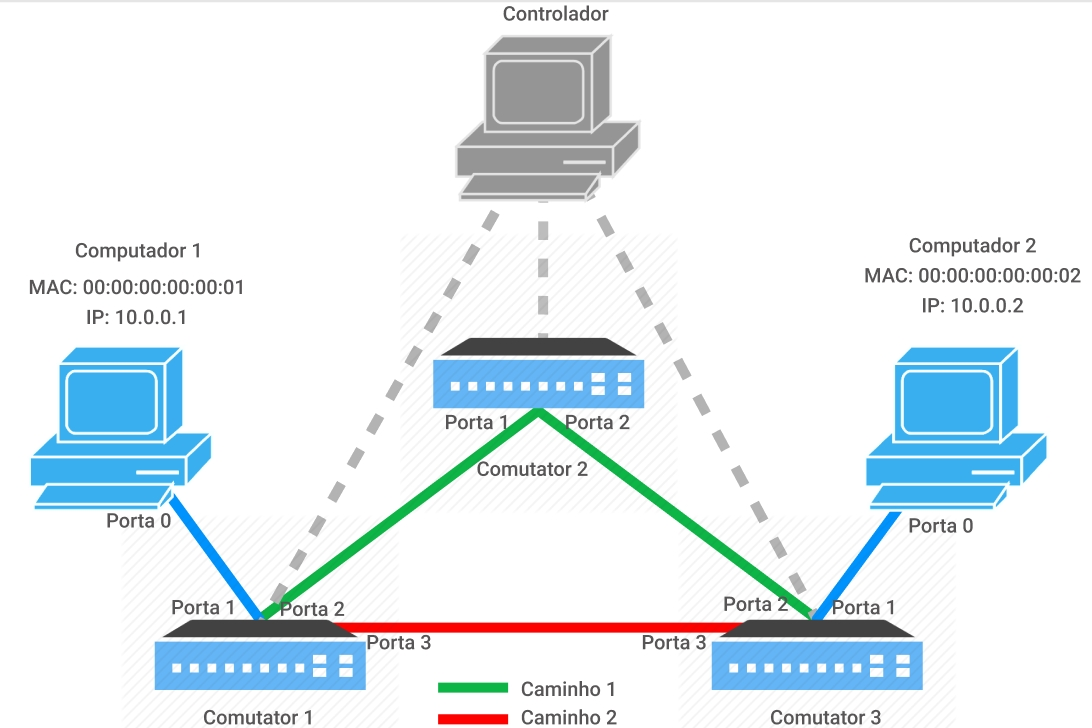
\includegraphics[scale=0.45]{imagens/topologia_explicacao.jpg}
	\end{center}
	\fonte{Elaborada pelo autor (2021).}
\end{figure}

A topologia ilustrada pela Figura \ref{fig:topo_explicacao}  contém dois caminhos possíveis entre o computador 1 e o computador 2. Essa topologia é utilizada para explicar o funcionamento das políticas de RR Seção~\ref{sec:rr}, CMCR Seção~\ref{sec:rf}, CMCP ~\ref{sec:pf} e CMT descrito na Seção~\ref{sec:bw}.

%https://books.google.com.br/books?id=Bc1qAAAAQBAJ&lpg=PT2&ots=nlGoe6R9A6&dq=software%20defined%20networking%20OSPF&lr&hl=pt-BR&pg=PT5#v=twopage&q&f=true

\section{Round-Robin}
\label{sec:rr}
A estratégia do RR é utilizar o algoritmo \emph{First In, First Out} (FIFO) para fazer o escalonamento entre caminhos que podem levar o pacote da origem até o destino, sendo  essa estratégia implementada de forma proativa. O algoritmo faz o balanceamento de novos fluxos criados, fazendo a redistribuição desses fluxos por caminhos alternativos em tempo real, dividindo a sobrecarga dos enlaces. 
Em sua estratégia mais clássica, toda vez que um pacote de um determinado fluxo gera um \textit{packet-in} no comutador, o controlador fica responsável por encontrar todos os caminhos de origem a destino e enfileirar estes caminhos em ordem, de tal forma que o caminho selecionado é removido do início e adicionado ao fim da fila. Este processo é repetido para cada novo \textit{packet-in} gerado, fazendo com que os servidores ao se comunicarem utilizem sempre múltiplos caminhos.

Quando o computador 1 da Figura~\ref{fig:topo_explicacao} executar o comando \textit{ping} ao endereço do computador 2 (\textit{e.g},10.0.0.2), antes de enviar os pacotes de sequência do protocolo ICMP, ele precisa do endereço MAC do destino, para isso é enviado um pacote ARP com MAC destino em \emph{broadcast}. Após a validação do MAC de destino as sequências dos pacotes ICMP começam a ser enviadas. A Figura ~\ref{fig:proxyArp} ilustra o percurso que este ARP realiza na política de RR para a topologia da Figura \ref{fig:topo_explicacao}. O evento 1 do diagrama é o envio do ARP \emph{broadcast} com o endereço MAC de destino ~\emph{FF:FF:FF:FF:FF:FF}. Um \emph{packet-in} é gerado no evento 2 para que o controlador decida a ação. Como o controlador tem a referência do destino é feito um ~\emph{proxy},  procedimento que  entrega o pacote diretamente para o comutador e porta vinculada ao endereço IP do destino, evento 3 e 4, ou possíveis destinos, quando o controlador não tem nenhuma referência conhecida. Nesta topologia, o computador 2 que é o destino, está ligado a porta 1 do comutador 3  . Então o evento 4 do diagrama irá enviar o pacote do \textit{packet-in}, diretamente ao comutador 3 com a ação \textit{output(1)}. O evento 5 ilustra o momento em que o pacote é enviado diretamente ao destino. 

Ao receber o pacote ARP que pergunta qual o MAC do endereço 10.0.0.2, o computador 2 é obrigado a responder com a mensagem \emph{10.0.0.2 at: 00:00:00:00:00:02}, porque este é seu endereço, representado na Figura \ref{fig:proxyArp} pelo evento 6. Caso o ARP entregue pelo controlador não corresponda o endereço, não seria gerado resposta. A resposta entregue ao comutador 3 não possui regras para tratar o pacote, gerando o evento 7 (\emph{packet-in}). Analisando o cabeçalho do pacote o controlador faz novamente o \emph{proxy} entregando diretamente ao comutador 1 para ser enviado pela porta 1 (evento 9 do diagrama). No evento 10 o comutador aplica a ação que veio junto ao pacote, entregando a resposta ao computador 1. Essa forma de resolução de ARP é a mesma para todas as políticas CMCP e CMT. O controlador não insere regra de fluxo durante o processamento de \textit{packet-in} gerado por pacotes ARP, para que o controlador possa comportar dispositivos móveis conectados a pontos de acesso \textit{wireless} de algumas SDN. Dessa forma, para manter a consistência da rede, após um limite de tempo ocioso, a referência que o controlador possui do dispositivo terminal é removida. Nesse caso em que o controlador não tem essa referência, o pacote é enviado para todas as portas que não são enlaces do tipo comutador-comutador, com intuito de encontrar o dispositivo terminal, ou seja, faz uma operação de \emph{proxy}, enviando o pacote para todas as conexões desconhecidas de modo a validar o endereço do computador. Esse formado de resolução de ARP também é útil em redes com múltiplos caminhos, pois entrega os pacotes ~\emph{broadcast} diretamente as portas de comutadores ligados a possíveis dispositivos terminais, evitando futuros \textit{packet-in} para o mesmo pacote. 


%%%%%%%%%%%%%%%%%%%%%%%%%%%%%%____FIGURA__RR___%%%%%%%%%%%%%%%%%%%%%%%%%%%%%%Grafo rede SDN.jpg
\begin{figure}[htb!]
	\caption{\label{fig:proxyArp}Diagrama de sequência, funcionamento da resolução de ARP das abordagens Proativas.} 
	\begin{center}
	    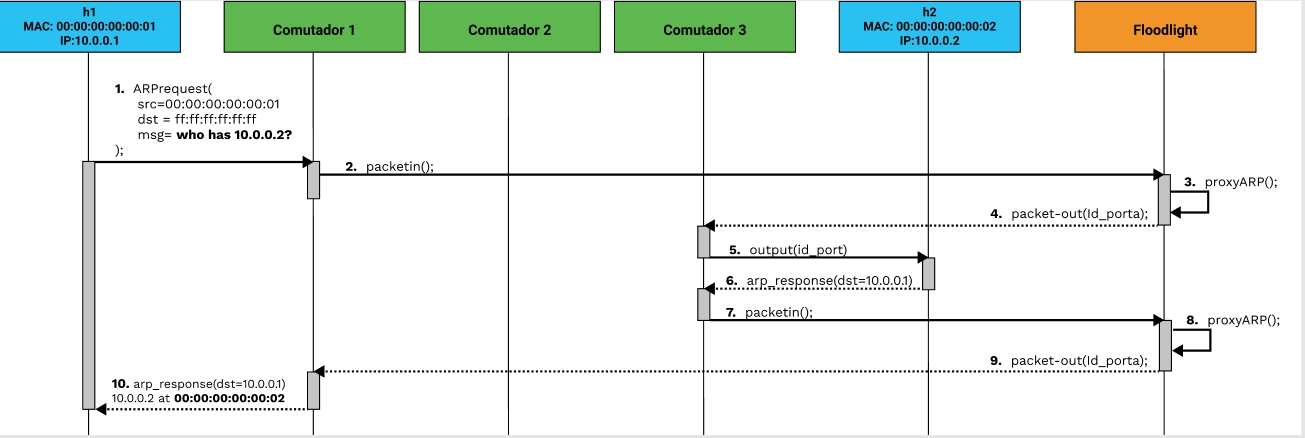
\includegraphics[scale=0.45]{imagens/arpProxy.jpg}
	\end{center}
	\fonte{Elaborada pelo autor (2021).}
\end{figure}

Depois que o ARP é resolvido no evento \textbf{10} do diagrama ilustrado pela Figura \ref{fig:proxyArp}, e o computador que está fazendo a requisição possui a validação do endereço de MAC do destino, então é iniciado o envio das sequências de pacotes. Como o controlador não inseriu nenhuma regra nas tabelas de fluxos dos comutadores, será disparado um \textit{packet-in} já no primeiro pacote. Então é iniciado os eventos começados na sequência \textbf{11} do diagrama da Figura ~\ref{fig:rr}.

\begin{figure}[htb!]
	\caption{\label{fig:rr} Diagrama de sequência, funcionamento da política de ~\emph{Round-Robin}.} 
	\begin{center}
	    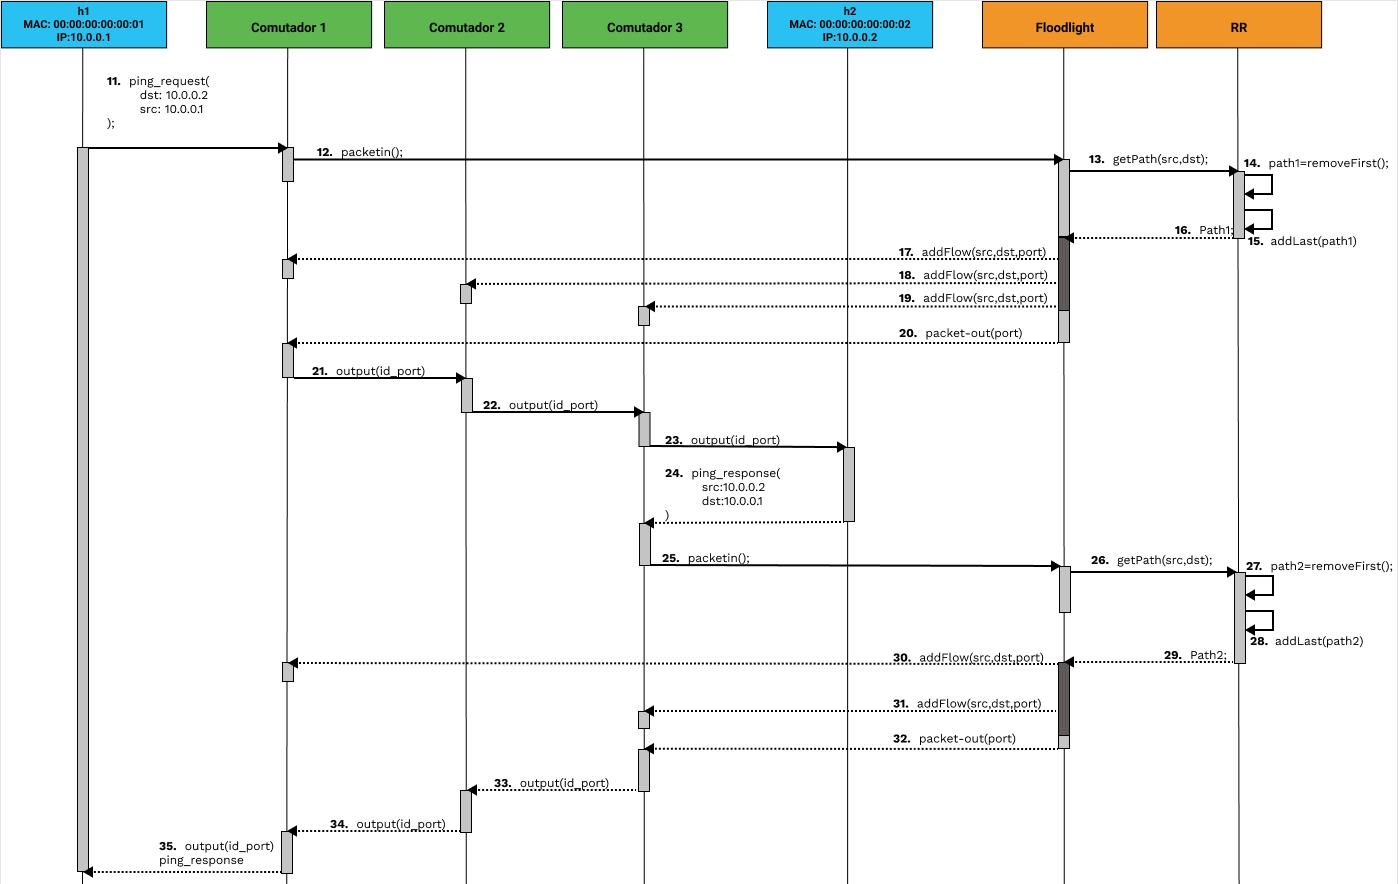
\includegraphics[scale=0.43]{imagens/rr.1.jpg}
	\end{center}
	\fonte{Elaborada pelo autor (2021).}
\end{figure}

O evento 11 é o envio do primeiro pacote ao comutador. No evento 12 o comutador identifica a falta de \emph{match} mara tratar o pacote, gerando um ~\textit{packet-in}. O eventro 13 ocorre com o controlador utilizando os endereços contidos no pacote para buscar o caminho entre origem e destino. Neste cenário  controlador possui dois caminhos enfileirados em um \textit{cache} interno, caminho 1 e caminho 2 da Figura \ref{fig:topo_explicacao}. O evento 14 pega o primeiro caminho nessa fila e o evento 15 passa esse caminho para o fim da fila, a referência do caminho é uma sub lista contendo tuplas de comutador/porta que são necessários configurar para o encaminhamento. 
Como nesse cenário o caminho 1 contém três comutadores, é criado um \emph{match} com as informações do pacote e enviado para o comutador 1, 2 e 3 da Figura \ref{fig:topo_explicacao}, representados no diagrama pelas sequências 17, 18 e 19. O evento 20 ocorre depois da configuração com o controlador devolvendo o pacote recebido no \emph{packet-in} ao comutador que o gerou. Os eventos 21, 22 e 23 são respectivos ao encaminhamento pela aplicação das regras que  determinam a porta de saída. O evento 24 é o momento em que o computador envia a seu comutador a resposta para a sequência 1 do comando \emph{ping}. No evento 25 é gerado outro \textit{packet-in} para tratar a volta do pacote. Passando diretamente ao evento 27, ao selecionar o caminho na fila, o primeiro da lista agora é o caminho 2. O evento 28 passa o caminho 2 ao final da fila e retorna a referência desse caminho contendo o comutador 1 e 3 da Figura \ref{fig:topo_explicacao}. O evento 30 e 31 são acionados para inserção das regras e ações nesses dois comutadores. A última ação do controlador é o evento 32, em que o pacote recebido é devolvido ao comutador que o enviou para seguir seu fluxo configurado. A partir deste ponto, os demais pacotes do fluxo são encaminhados conforme a configuração. Se o fluxo não receber pacotes durante 5 segundos, especificado no contador \textit{idl\_time} o comutador remove o fluxo.


\section{Caminho mais curto reativo}
\label{sec:rf}
A política CMCR faz o encaminhamento pela rota com menor quantidade de comutadores entre origem e destino reativamente, configurando um comutador por vez, ou seja, quando o controlador recebe o \textit{packet-in} ele configura o comutador que o gerou para que o pacote seja encaminhado para o próximo salto. A resolução do ARP nessa política ocorre conforme o diagrama da Figura \ref{fig:rf1}, já os pacotes gerados após a resolução de ARP são ilustrados pela Figura~\ref{fig:rf2}. O cenário utilizado para exemplificar o funcionamento desse algoritmo é o mesmo da Figura \ref{fig:topo_explicacao}.

Antes de iniciar o envio de pacotes da sequência \textit{ping}, o computador 1 precisa do endereço MAC de destino. A forma como a política reativa trata os ARPs \textit{broadcast} é muito similar as redes convencionais. Quando o controlador precisa que um comutador realize um \emph{broadcast}, é adicionado a ação \emph{flood} na construção de um \emph{packet-out}. O \textit{flood} é uma especificação interna do \textit{Openflow}, em que o comutador faz uma cópia do pacote para cada porta de um subconjunto de portas permitidas. Ou seja, portas reservadas, bloqueadas e a porta controlador não são utilizadas na execução do \emph{flood}. 

O primeiro evento ilustrado na Figura \ref{fig:rf1} é o envio da solicitação do endereço MAC do destino. O evento 2 é gerado o \textit{packet-in} pela falta de regras. Como o controlador está utilizando a política de controle de fluxo reativa precisa manter um  \emph{cache} atualizado que contém informações do comutador e os \textit{packet-in} que ele já enviou, para evitar o afogamento dos enlaces gerados em ciclos no plano de dados. Esse controle é representado no evento 3 do diagrama ilustrado pela Figura \ref{fig:rf2}, na qual, o controlador verifica no \textit{cache} do comutador 1 se este pacote já passou uma vez por ele, como é a primeira vez a verificação é falsa, então o pacote é adicionado ao \textit{cache} com o identificador do comutador 1. Após guardar a referência o controlador insere a regra no comutador (evento 6) e devolve o pacote recebido pelo \emph{packet-in} com uma ação \emph{flood}.

\begin{figure}[htb!]
	\caption{\label{fig:rf1} Diagrama de sequência, resolução de ARP na política de encaminhamento reativa.} 
	\begin{center}
	    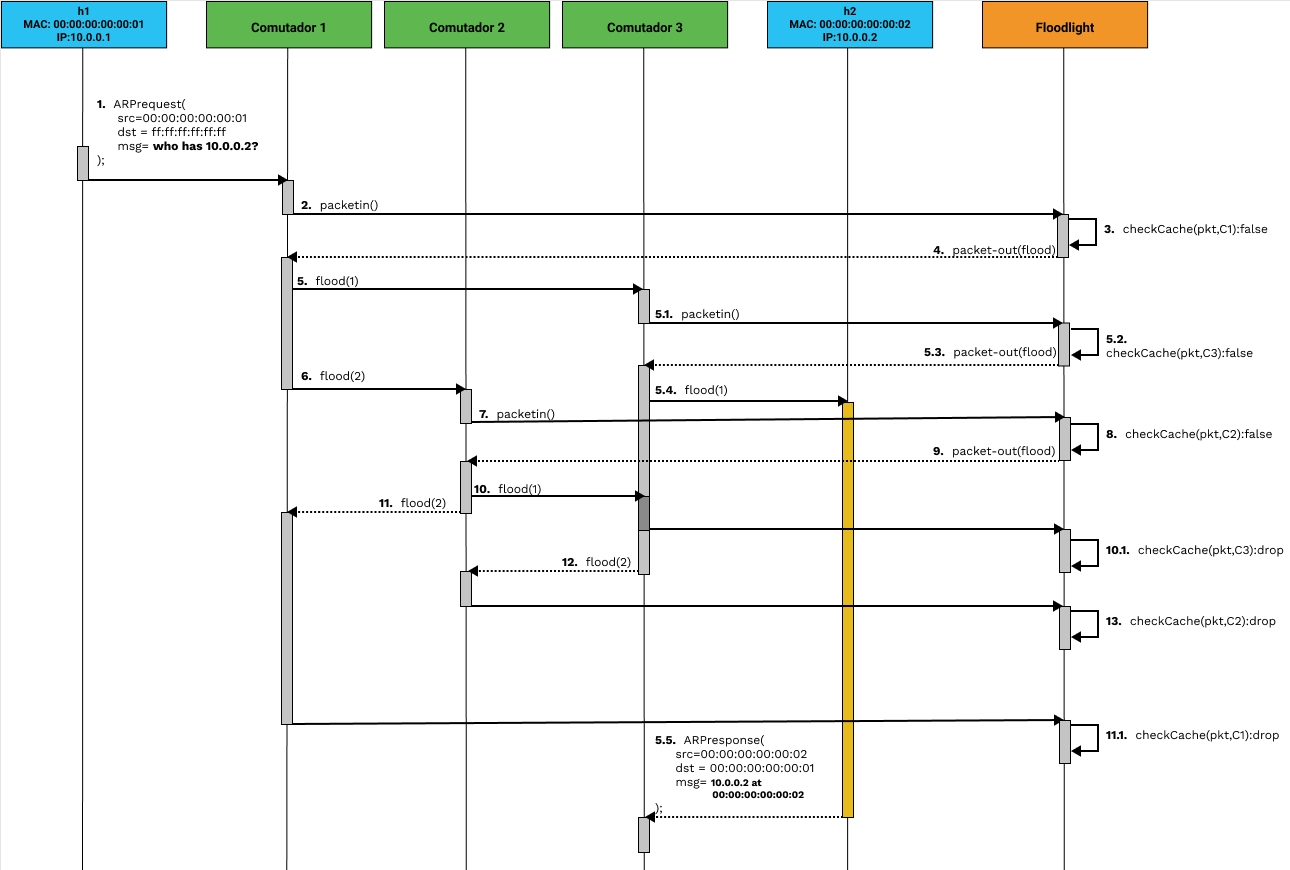
\includegraphics[scale=0.43]{imagens/rf.jpg}
	\end{center}
	\fonte{Elaborada pelo autor (2021).}
\end{figure}

\begin{figure}[htb!]
	\caption{\label{fig:rf2} Diagrama de sequência, funcionamento do caminho mais curto na abordagem reativa.} 
	\begin{center}
	    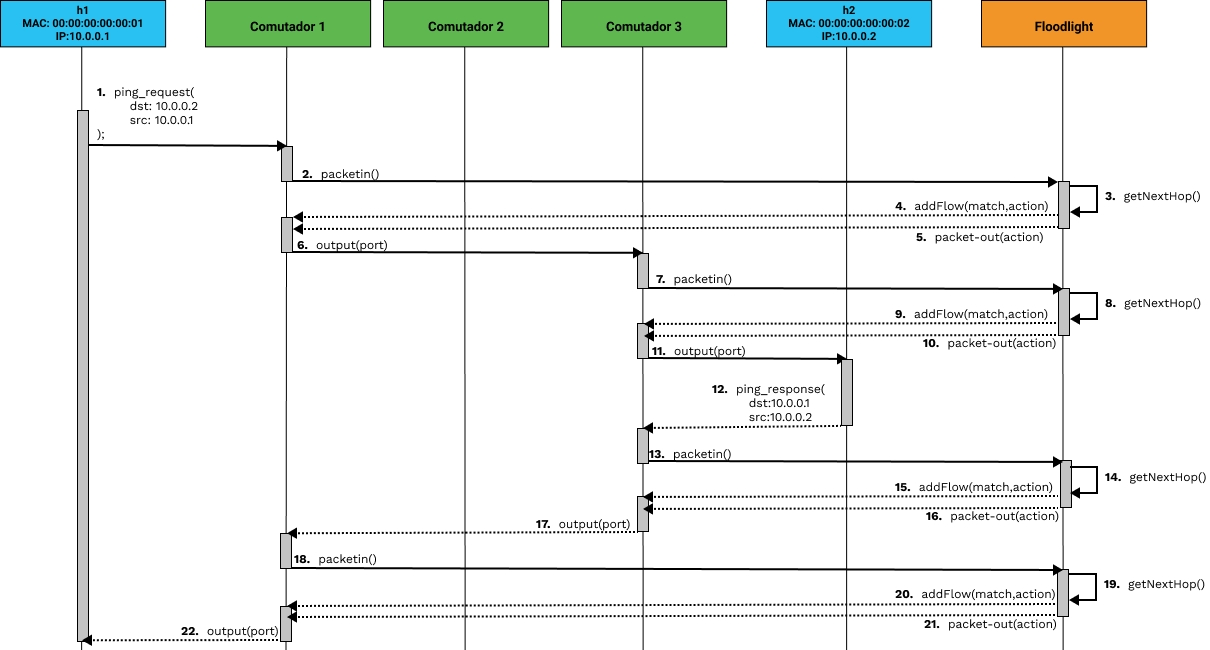
\includegraphics[scale=0.43]{imagens/rf.2.jpg}
	\end{center}
	\fonte{Elaborada pelo autor (2021).}
\end{figure}
Ao processar a instrução \emph{flood} recebida do controlador, o comutador faz a cópia do pacote e o envia para todas as portas válidas, que neste cenário é representada pelos eventos 5 e 6. A partir desse momento o pacote é processado em paralelo pelo comutador 2 e o comutador 3, pois cada um possui uma cópia do pacote.  Os eventos 5.1 e 7 são \emph{packet-in} resultante do recebimento dos pacotes gerados pelo \emph{flood}. O evento 5.2 faz uma verificação do pacote no comutador 3, enquanto o evento 8 realizado em paralelo faz a verificação do pacote no comutador 2. Ambos estão sendo processados pela primeira vez em cada comutador, portanto suas referências são armazenadas no \textit{cache} com a identificação de seus respectivos comutadores. Novamente o controlador irá fazer o \emph{flood} desses pacotes, eventos 5.3 e 9. Quando o comutador 3 realiza a operação de \emph{flood}, uma das portas entrega o pacote ao destino, enquanto a outra porta entrega o pacote ao comutador 2, representado na figura pelo evento 12. 

Quando o controlador analisar o \emph{packet-in} gerado pelo comutador 2 no evento 13, é verificado no \textit{cache} que este pacote já passou uma vez por este comutador, portanto pode ser descartado. Caso esse controle não seja feito, os ciclos no plano de dados clonariam os pacotes indefinidamente. O pacote entregue ao computador pelo evento 5.4 gera a resposta do evento 5.5, assim todo o processo é novamente iniciado para que o pacote volte para origem da requisição. O \textit{cache} do controlador responsável por armazenar a referência dos \textit{packet-in} já processados por cada comutador, possuem um tamanho fixo e as referências mais antigas são descartadas para evitar uso excessivo de memória. 


Após os eventos de pacotes ARP o solicitante envia os pacotes do \emph{ping} com os endereços do destino. A figura \ref{fig:rf2} ilustra o encaminhamento desses pacotes utilizando a política reativa. O evento 1 corresponde ao envio ao comutador, gerando o \emph{packet-in} por falta de regra no evento 2. O controlador busca na topologia interna representada pelo grafo qual o próximo salto do caminho de menor número de saltos, representado pelo evento 3 do diagrama. Como esta política considera apenas um salto, é inserido a regra de fluxo no evento 4 e devolvido o pacote ao comutador no evento 5. O evento 6 representa o encaminhamento para o próximo nó da rede, o comutador 3.
Um novo \emph{packet-in} é gerado no evento 7 repetindo as ações de configuração que consiste em encontrar o próximo salto, configurar o comutador e devolver o pacote, evento 8, 9 e 10. No evento 11 a aplicação da regra sobre o pacote faz a entrega diretamente ao destino. 

O procedimento realizado para o pacote de origem 10.0.0.2 para 10.0.0.1 segue a mesma lógica anterior, eventos de 13 a 22 correspondem a criação de um novo fluxo para que a resposta volte a origem da solicitação. 
%%

\section{Caminho mais curto proativo}
\label{sec:pf}

A política CMCP, utiliza a rota com menor quantidade de saltos entre origem e destino, configurando todos os saltos no primeiro \textit{packet-in}. Considerando o mesmo cenário de exemplo dos algoritmos anteriores, Figura \ref{fig:topo_explicacao}, mesmo que tenha caminhos alternativos o controlador sempre irá escolher o mesmo caminho para criar o fluxo de ida e o fluxo de volta. 

\begin{figure}[htb!]
	\caption{\label{fig:pf} Diagrama de sequência, funcionamento da política de caminho mais curto da abordagem proativa.} 
	\begin{center}
	    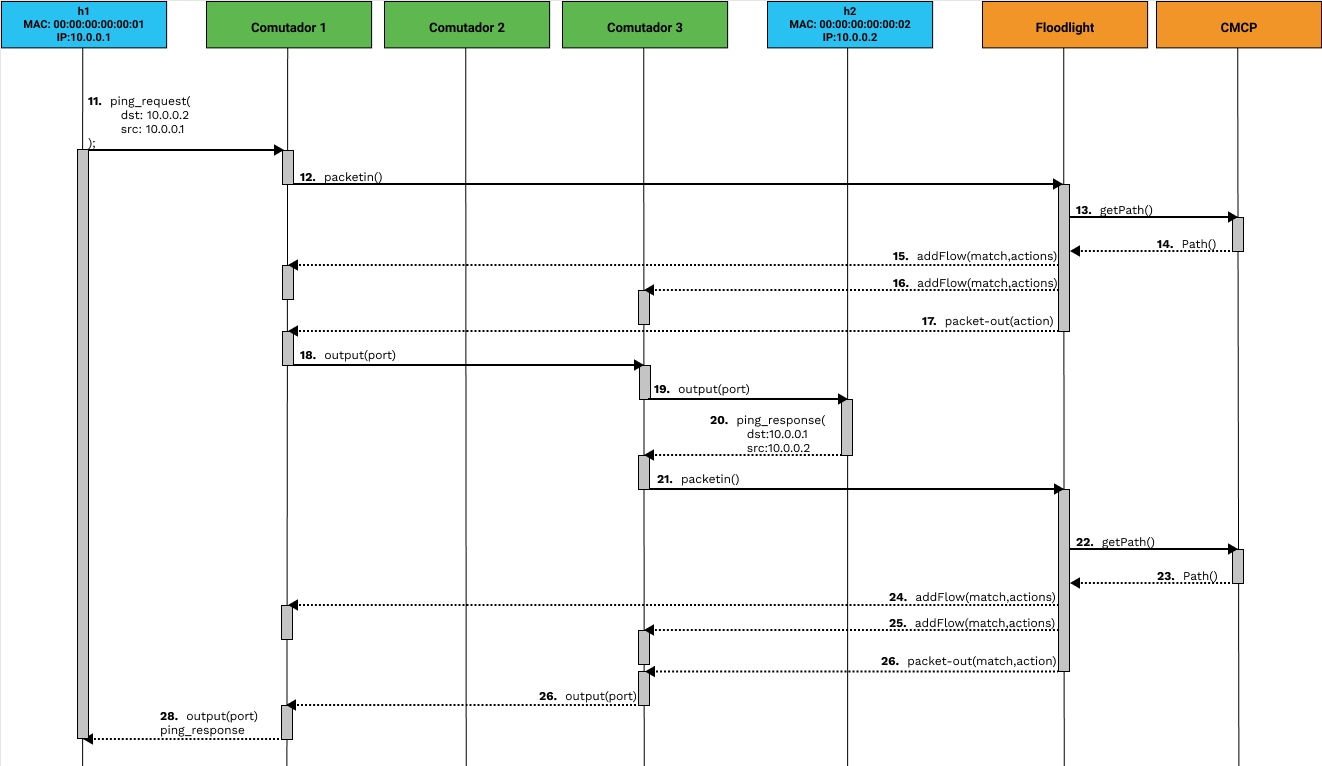
\includegraphics[scale=0.43]{imagens/pf.jpg}
	\end{center}
	\fonte{Elaborada pelo autor (2021).}
\end{figure}
A figura \ref{fig:pf} ilustra o funcionamento da política de encaminhamento para o tráfego gerado pelo comando \emph{ping}. Logo apos os eventos de resolução de ARP usando o \textit{proxy} da Figura \ref{fig:proxyArp}, o próximo evento é iniciado em 11, com a chegada do primeiro pacote da sequência ICMP. Sendo o primeiro pacote o comutador não possui regras em sua tabela para o encaminhamento, gerando o \emph{packet-in} representado na figura pelo evento 12. Ao receber o pacote o controlador faz uma busca no grafo interno que representa a topologia, ilustrado pelo evento 13. Como o grafo tem dois possíveis caminhos, a topologia retorna uma lista ordenada pela quantidade de comutadores em cada caminho, da qual o primeiro da lista é o que possui menor numero de saltos e esta representado pelo evento 14 do diagrama. 

Com as informações de comutadores e portas o controlador gera o \emph{match} com ações para cada elemento do caminho e adiciona essas regras nos comutadores, eventos 15 e 16. Após a inserção das regras o controlador devolve o pacote ao comutador que o enviou junto a uma ação de porta de saída, evento 17. A partir deste ponto o pacote segue o fluxo até o destino, evento 18, 19. 
A resposta gerada pelo destino cria um \emph{packet-in} no evento 21. Como o controlador utilizara novamente o primeiro caminho da lista de caminhos, os comutadores que receberão as regras de fluxo são os mesmos que utilizados anteriormente, eventos 24 e 25. O controlador devolve o pacote no evento 26 para seguir o fluxo,  entregando a resposta do \emph{ping} ao solicitante no evento 28.  
Este algorítimo possui o funcionamento mais simples que os demais, porém utiliza o mesmo caminho mais vezes.



\section{Caminho de menor tráfego}
\label{sec:bw}
Os comutadores que utilizam o protocolo \textit{Openflow} fornecem diversas informações sobre os dispositivos. As informações como bits transmitidos e enviados por cada portas podem ser medias periodicamente para se obter estatísticas como taxa de transferência e assim identificar os enlaces que estão sendo menos utilizados. Tal informação permite a criação de algoritmos que calcula o tráfego de todas as rotas existentes entre origem e destino, assim quando o controlador faz a requisição da rota de menor tráfego esta informação já se encontra pronta para uso.
\begin{figure}[!htb]
	\caption{\label{fig:bw_1}Diagrama de sequência, funcionamento da política de caminho de menor tráfego.}
	\begin{center}
	    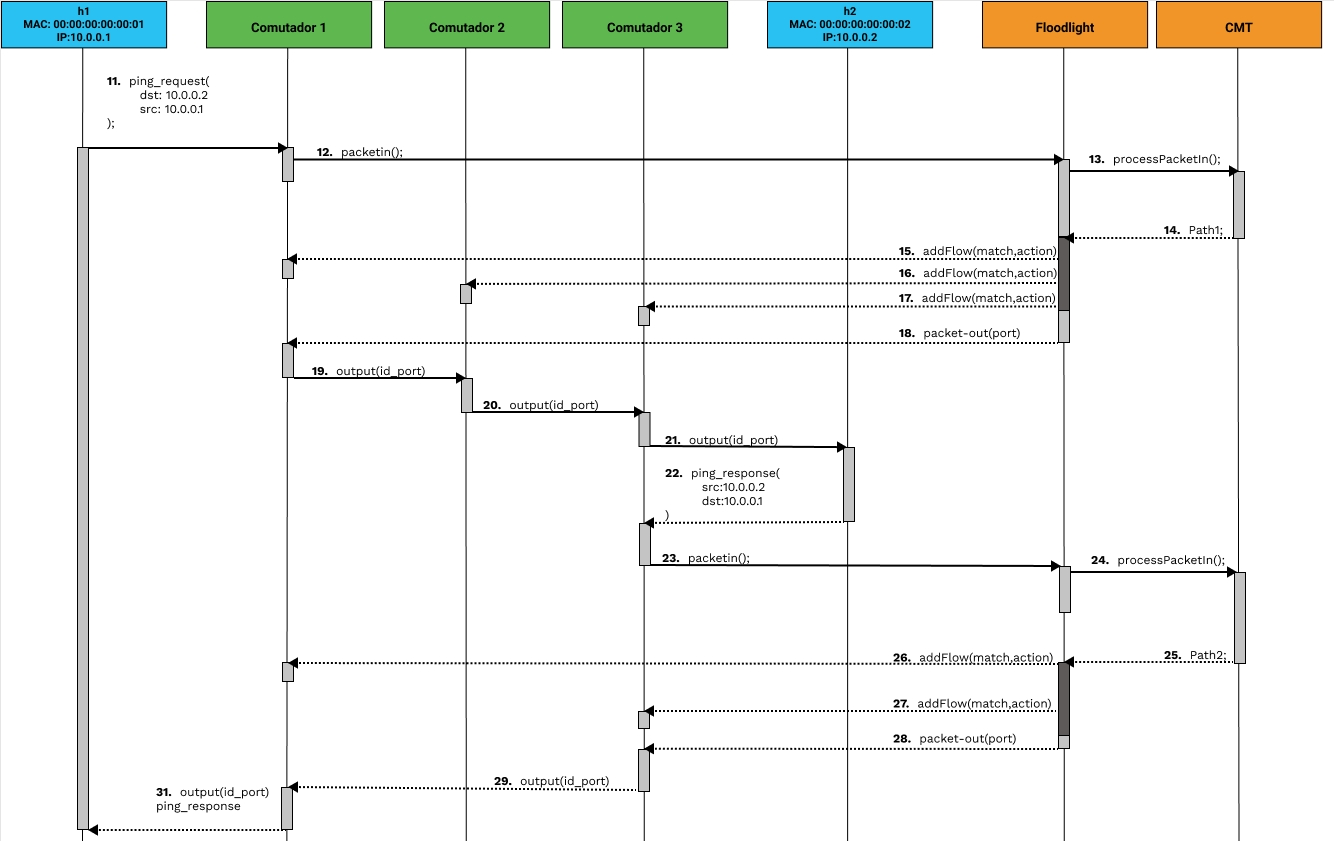
\includegraphics[scale=0.445]{imagens/bw.1.jpg}
	\end{center}
	\fonte{Elaborada pelo autor (2021).}
\end{figure}

\begin{figure}[!htb]
	\caption{\label{fig:bw_2}Diagrama de sequência, troca de informações internas no algoritmo de caminho de menor tráfego.}
	\begin{center}
	    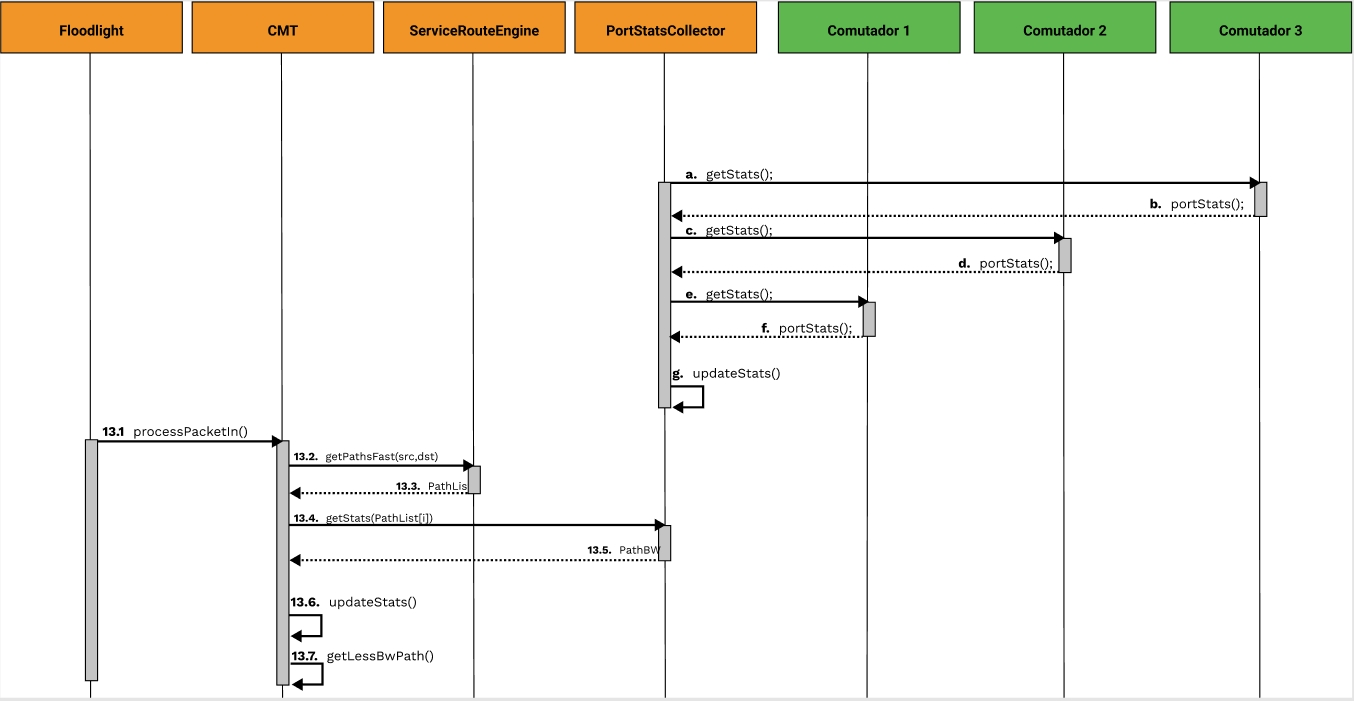
\includegraphics[scale=0.445]{imagens/bw.2.jpg}
	\end{center}
	\fonte{Elaborada pelo autor (2021).}
\end{figure}
A Figura ~\ref{fig:bw_1} ilustra o funcionamento do algoritmo para o envio de um pacote entre ~\textit{~\textbf{h1}} e ~\textit{~\textbf{h2}} com o comando ~\textit{ping} no plano de dados representado pela Figura~\ref{fig:topo_explicacao}. Diferente do algoritmo que considera a quantidade de saltos como caminho mais curto, este utiliza a soma de dados transferidos por cada enlaces do caminho para encontrar qual tem o menor trafego. Caso o caminho 1 que possui maior número de saltos apresente menor utilização de enlaces este é selecionado como caminho de menor tráfego. A vazão total do tráfego é limitado pelo enlace entre o comutador e o computador. Ou seja, se esse enlace é de \textit{1 Gb/s} então mesmo que existam rotas alternativas entre os comutadores não é possível que essa velocidade seja superada.   
O diagrama da Figura ~\ref{fig:bw_1} possui troca de informações divididas em três cores. Em azul estão os computadores, em cor verde os comutadores e em laranja as classes internas do \textit{Floodlight} que foram expandidas na Figura ~\ref{fig:bw_2} com maiores detalhes. Os eventos da figura ~\ref{fig:bw_1} começam na sequência 11 após a resolução de pacotes ARPs, e terminam na sequência 31, com a resposta do comando ~\textit{ping}. Os eventos da Figura ~\ref{fig:bw_2} que vão da sequência 13.1 à 13.7 ocorrem entre os eventos 13 e 14 da Figura ~\ref{fig:bw_1}. 


\begin{table}[!htb]
\centering
\caption{Descrição dos eventos usados para configuração do fluxo na política de menor tráfego.}
\label{tab:bw}
\begin{tabular}{lllll}
\cline{1-2}
\multicolumn{1}{|l|}{\textbf{Evento}} & \multicolumn{1}{l|}{\textbf{Descrição}} &  &  &  \\ \cline{1-2}
\multicolumn{1}{|l|}{11. ping request} & \multicolumn{1}{l|}{\begin{tabular}[c]{@{}l@{}}O primeiro pacote da sequência \textit{ping} já contendo os endereços\\  resolvidos pelo ARP é enviado para o comutador\end{tabular}} &  &  &  \\ \cline{1-2}
\multicolumn{1}{|l|}{12. packetin} & \multicolumn{1}{l|}{\begin{tabular}[c]{@{}l@{}}Como o comutador não possui regra de match para o cabeçalho \\ do pacote, este é enviado ao controlador\end{tabular}} &  &  &  \\ \cline{1-2}
\multicolumn{1}{|l|}{13. processPacketIn} & \multicolumn{1}{l|}{\begin{tabular}[c]{@{}l@{}}O controlador desenpacota a menssagem na qual são extraidas\\  as informações necessárias\end{tabular}} &  &  &  \\ \cline{1-2}
\multicolumn{1}{|l|}{13.2 getPathFast} & \multicolumn{1}{l|}{\begin{tabular}[c]{@{}l@{}}Busca em um grafo/cache local todos os caminhos possíveis \\ entre origem e destino\end{tabular}} &  &  &  \\ \cline{1-2}
\multicolumn{1}{|l|}{13.4 getStats} & \multicolumn{1}{l|}{\begin{tabular}[c]{@{}l@{}}Para cada caminho existente é buscado a soma do trafego entre\\  os enlaces\end{tabular}} &  &  &  \\ \cline{1-2}
\multicolumn{1}{|l|}{13.6 updateStats} & \multicolumn{1}{l|}{A lista é ordenada de forma crecente de tráfego} &  &  &  \\ \cline{1-2}
\multicolumn{1}{|l|}{13.7 getLessBwPath} & \multicolumn{1}{l|}{\begin{tabular}[c]{@{}l@{}}Seleciona o caminho de menor tráfego, gerando uma lista de \\ tuplas com comutador e porta\end{tabular}} &  &  &  \\ \cline{1-2}
\multicolumn{1}{|l|}{15, 16, 17. addFlow} & \multicolumn{1}{l|}{\begin{tabular}[c]{@{}l@{}}É gerado um match com as informações do pacote, cada \\ elemento da lista de tuplas tem sua respectiva ação relacionada a \\ porta de saída. As regras são então enviadas aos comutadores\end{tabular}} &  &  &  \\ \cline{1-2}
\multicolumn{1}{|l|}{18. packet Out} & \multicolumn{1}{l|}{\begin{tabular}[c]{@{}l@{}}Realizado após a adição dos fluxos no switch, devolve o pacote \\ novamente ao comutador que gerou o packet-in para que ele siga\\  o fluxo configurado\end{tabular}} &  &  &  \\ \cline{1-2}
\multicolumn{1}{|l|}{19, 20, 21} & \multicolumn{1}{l|}{\begin{tabular}[c]{@{}l@{}}Comutadores aplicam as ações relacionada ao match instalado\\  anteriormente\end{tabular}} &  &  &  \\ \cline{1-2}
\multicolumn{1}{|l|}{22. ping\_response} & \multicolumn{1}{l|}{O computador de destino envia a resposta para o request} &  &  &  \\ \cline{1-2}
\multicolumn{1}{|l|}{23. packetin} & \multicolumn{1}{l|}{\begin{tabular}[c]{@{}l@{}}Como o controlador configurou apenas a rota de 10.0.0.1 para \\ 10.0.0.2, agora é necessário gerar as regras para tratar pacotes de \\ 10.0.0.2 para 10.0.0.1\end{tabular}} &  &  &  \\ \cline{1-2}
\multicolumn{1}{|l|}{31. ping\_response} & \multicolumn{1}{l|}{A resposta do \textit{ping} é entregue ao solicitante} &  &  &  \\ \cline{1-2}
\cline{1-2}
\multicolumn{1}{|l|}{\textbf{Evento}} & \multicolumn{1}{l|}{\textbf{Descrição}} &  &  &  \\ \cline{1-2}
\multicolumn{1}{|l|}{a,c,e} & \multicolumn{1}{l|}{\begin{tabular}[c]{@{}l@{}}Controlador envia para cada comutador da rede uma solicitação\\  de estatísticas.\end{tabular}} &  &  &  \\ \cline{1-2}
\multicolumn{1}{|l|}{b,d,f} & \multicolumn{1}{l|}{\begin{tabular}[c]{@{}l@{}}Pacotes enviados dos comutadores contendo todas as estatísticas \\ de portas e entradas da tabela de fluxo.\end{tabular}} &  &  &  \\ \cline{1-2}
\multicolumn{1}{|l|}{g} & \multicolumn{1}{l|}{\begin{tabular}[c]{@{}l@{}}As informações são atualizadas em um cache interno para consulta\\  de consumo de comutador/porta\end{tabular}} &  &  &  \\ \cline{1-2}
 &  &  &  &  \\
 &  &  &  & 
\end{tabular}
\fonte{Elaborada pelo autor (2021).}
\end{table}

A Tabela ~\ref{tab:bw} possui uma descrição detalhada sobre os principais eventos que ocorrem para a configuração de um novo fluxo conforme a política de menor tráfego. Sendo que os eventos de ~\textbf{a} até ~\textbf{g} são tarefas paralelas executadas periodicamente a cada segundo, esses são responsáveis por manter a taxa de utilização dos enlaces, calculados e armazenados no \textit{cache} interno do controlador para consultas, de modo a minimizar o tempo de resposta ao \textit{packet-in}. 

\section{Trabalhos Relacionados}
\label{sec:trabalhos_relacionados}
Foram encontrados na literatura seis trabalhos relacionados a avaliação e comparação de políticas de controle de fluxo em SDN. A Tabela \ref{tab:trabalhos_relacionados} traz um levantamento sobre as políticas, métricas de avaliação, topologias e ambientes utilizados para comparação dos algoritmos.

%%%%%%%%%%%%%%%%%%%%%%%%%%%%%%%%%%%%%%%%%%%%%%%%%%%%%
% Please add the following required packages to your document preamble:
% \usepackage{graphicx}
% \usepackage{lscape}
% Please add the following required packages to your document preamble:
% \usepackage{graphicx}
% \usepackage{lscape}
\begin{table}[]
\centering
\caption{Trabalhos relacionados a comparações de políticas de encaminhamento de fluxo.}
\label{tab:trabalhos_relacionados}
\resizebox{\textwidth}{!}{%
\begin{tabular}{lllll}
\hline
\textbf{Referências} &
  \textbf{Algoritmos} &
  \textbf{Métricas} &
  \textbf{Topologia} &
  \textbf{Ambiente} \\ \hline
\cite{akin2019comparison} &
  \begin{tabular}[c]{@{}l@{}}Classe 1:\\ 1. \textit{Minimum Hop Algorithm} (MHA);\\ 2. \textit{Shortest Path}  (SP);\\ 3. \textit{Widest-Shortest Path} (WSP).\\ \\ Classe 2:\\ 1. \textit{Dynamic Shortest Path} (DSP);\\ 2. \textit{Dynamic Widest-Shortest Path} (DWSP).\\ \\ Classe 3:\\ 1. \textit{Minimum Interference Routing}\\ \textit{Algorithm}~(MIRA);\\ 2. \textit{Least Interference}\\ \textit{Optimization Algorithm}~(LIOA);\\ 3. \textit{Improved Least Interference}\\ \textit{Optimization Algorithm}~(ILIOA).\end{tabular} &
  \begin{tabular}[c]{@{}l@{}}1. Total de dados transferidos(\textit{throughput});\\ 2. Quantidade de pacotes perdidos;\\ 3. Tempo de computação do caminho.\end{tabular} &
  \begin{tabular}[c]{@{}l@{}}1. \textit{MIRANET};\\ 2. \textit{ANSNET};\end{tabular} &
  \begin{tabular}[c]{@{}l@{}}Plano de controle: RYU;\\ Plano de dados: \textit{Mininet}.\end{tabular} \\ \hline
\cite{ichikawa2013network} &
  \begin{tabular}[c]{@{}l@{}}1.  \textit{Warshall-Floyd}  (Proposta);\\ 2. \textit{Shortest Path};\end{tabular} &
  \begin{tabular}[c]{@{}l@{}}1. Total de dados transferidos (\textit{Throughput});\\ 2. Tempo de execução do NAS.\end{tabular} &
  \begin{tabular}[c]{@{}l@{}}1. Topologia intra-domínio: \\ (EUA, Japão, Singapura, Tailândia)\end{tabular} &
  \begin{tabular}[c]{@{}l@{}}Plano de controle: Não especificado;\\ Plano de dados: \textit{Open vSwitches}.\end{tabular} \\ \hline
\cite{naeem2020sdn} &
  \begin{tabular}[c]{@{}l@{}}1. \textit{Shortest Path};\\ 2. \textit{Lagrangian relaxation-based}\\ \textit{aggregated cost} (LARAC);\\ 3. Sway;\\ 2. SEQOS baseado \\ em \textit{Bellman–Ford}; (Proposta).\end{tabular} &
  \begin{tabular}[c]{@{}l@{}}1. Custo energético;\\ 2. Total de dados transferidos (\textit{Throughput}).\end{tabular} &
  \begin{tabular}[c]{@{}l@{}}1. \textit{Goodnet};\\ 2. \textit{AttMpls}.\end{tabular} &
  \begin{tabular}[c]{@{}l@{}}Plano de controle:  POX;\\ Plano de dados: \textit{Mininet}.\end{tabular} \\ \hline
\cite{casas2020intelligent} &
  \begin{tabular}[c]{@{}l@{}}1. \textit{Reinforcement Learning and}\\
\textit{Software-Defined Networking} \\ \textit{Intelligent Routing}~(RSIR);\\ 2. Shortest Path (Dijkstra):\\ 2.1. Tráfego;\\ 2.2. Taxa de perda de pacotes;\\ 2.3. Latência;\\ 2.4. Composto (Latencia + Perda + Vazão).\end{tabular} &
  1. Total de dados transferido (Throughput); &
  1. GÉANT: 23 comutadores. &
  \begin{tabular}[c]{@{}l@{}}Plano de controle: Ryu;\\ Plano de dados: Mininet.\end{tabular} \\ \hline
\cite{marcondes2016executing} &
  \begin{tabular}[c]{@{}l@{}}1. Shortest Path;\\ 2. Random Selection;\\ 3. Round-Robin over Multiple Paths;\end{tabular} &
  1. Tempo de execução do NAS. &
  \begin{tabular}[c]{@{}l@{}}1. Fat Tree: 8 servidores e \\ 10 comutadores.\end{tabular} &
  \begin{tabular}[c]{@{}l@{}}Plano de controle: Floodlight;\\ Plano de dados: Mininet.\end{tabular} \\ \hline
\cite{zhang2015performance}&
  \begin{tabular}[c]{@{}l@{}}1. Open Short Path First (OSPF) \\- redes tradicionais;\\ 2. Shortest Path - SDN.\end{tabular} &
  1. Tempo de resposta das requisições. &
  \begin{tabular}[c]{@{}l@{}}1. Topologia de 16 comutadores;\\ 2. Topologia de 120 comutadores.\end{tabular} &
  \begin{tabular}[c]{@{}l@{}}1. Rede tradicional:\\ 1.1. Controle: Quagga;\\ 1.2. Mininext.\\ \\ 2. SDN\\ 2.1. Plano de controle: Floodlight;\\ 2.2. Plano de dados: Mininet.\end{tabular} \\ \hline
\end{tabular}%
}
\fonte{Elaborada pelo autor (2021).}
\end{table}



%%%%%%%%%%%%%%%%%%%%%%%%%%%%%%%%%%%%%%%%%%%%%%%%


Em \cite{akin2019comparison}, foi efetuado um estudo de modo a poder comparar a eficiência entre três classes de algoritmos para controle de fluxo, algoritmos de encaminhamento com: 1) custo de enlace estático, 2) custo do enlace dinâmico e 3) custo do enlace dinâmico com interferência mínima. Na primeira classe contém tês algoritmos de encaminhamento que consideram custo estático como quantidade de saltos. A segunda classe possui duas variações para o caminho mais curto dinâmico, em que é utilizado largura de banda para calcular os pesos de enlaces. A terceira classe contém três algoritmos que adicionam pesos a enlaces criticos junto aos pesos de custo dinâmico. O trabalho comparou essas classes e concluiu que algorítimos dinâmicos tem um desempenho melhor que os estáticos, mas não possuem vantagens significativas entre si dentro de sua própria classe. Em relação à coleta de estatísticas da rede para os algoritmos de custo dinâmico, os autores destacaram duas abordagens. Uma busca manter a projeção atualizada da camada de dados no controlador de modo que o controlador tenha informações o suficiente para identificar os caminhos mais utilizados e estimar largura de banda. A outra abordagem para coleta de informações é fazer leituras periódicas dos comutadores. Esta última abordagem foi utilizada na política de CMT apresentada na Seção \ref{sec:bw}, e os desafios encontrados por este forma leitura são descritos em maiores detalhes na Seção \ref{sec:discussao_resultados}. 

Em \cite{ichikawa2013network} o autor propõe um agente para monitorar informações de latência e vazão permitindo o controlador aplicar no algoritmo de \textit{Warshall-Floyd} e encontrar o melhor caminho. Para validar a proposta o autor utilizou o programa \textit{Numerical Aerodynamic Simulation} (NAS) descrito em detalhes na Seção \ref{sec:aplicacao_teste_nas}. O resultado obtido pelo tempo de execução das aplicações foram comparados com os resultados obtidos pela política de menor caminho e concluiu que a solução proposta teve um desempenho melhor. 

Em \cite{naeem2020sdn}, o autor faz um estudo comparativo entre políticas de controle de fluxo em relação à eficiência do gasto de energia para \textit{Industrial Internet of Things} (IIoT). O autor considera para um bom gerenciamento do tráfego a perda de pacotes, \textit{jitter} e latência em relação ao QoS. O trabalho está relacionado a engenharia de tráfego e demostra como uma decisão tomada no plano de controle pode resolver das mais diferentes categorias de problemas apenas na forma como efetua o gerenciamento. Os resultados do autor mostra que é possível atingir uma redução de até 50\% do custo energético violando apenas 5\% do \textit{Service Level Agreement}~(SLA), resultado aceitável quando se trata de IIoT.

Ainda relacionado a alternativas de algoritmos de encaminhamento, o trabalho de \cite{casas2020intelligent} utiliza roteamento com aprendizagem por reforço como alternativa a gerenciamento do controle de fluxo. A proposta faz leituras periódicas de estatísticas do plano de dados para alimentar um novo plano acima do plano de gerenciamento, chamada \textit{ Knowledge Plane}, que extrai e analisa esses dados gerando o caminho ótimo, na qual, é considerado tanto a largura de banda, perda de pacotes e latência durante a avaliação dos caminhos. Para comparação da proposta o autor utilizou variações do algoritmo de \textit{Dijkstra}~\footnote{Dijkstra é um algoritmo eficiente para encontrar o caminho mais curto em um grafo com pesos em aresta.}, cada uma dessas variações foram baseadas em latência, perda de pacotes, largura de banda e ainda uma versão composta entre latência e largura de banda. A proposta apresentou melhor eficiência ao comparado com o \textit{Dijkstra} latência e \textit{Dijkstra} perda de pacotes, porém teve 3\% a menos de eficiência em relação ao \textit{Dijkstra} com largura de banda.

Em \cite{marcondes2016executing}, o autor compara a política de \textit{Shortest Path} com as políticas de \textit{Random Selection} que escolhe o caminho de forma aleatória, e a política de \textit{Round-Robin over Multiple Paths} cujo funcionamento é baseado em fila circular para escalonamento de caminhos, apresentado na Seção~\ref{sec:rr}. O autor cria uma topologia \textit{Fat Tree} com 8 servidores e 10 comutadores utilizando o \textit{mininet}. Para comparar as políticas utilizou o \textit{framework} NAS e com o tempo de execução das aplicações foi possível identificar que a utilização do \textit{Shortest Path} induz a criação de gargalos na camada de dados. Dessa forma o algoritmo \textit{Round-Robin over Multiple Paths} teve melhores resultados. O desempenho dos algoritmos de múltiplos caminhos são discutidos com mais detalhes na discussão dos resultados Seção \ref{sec:discussao_resultados}.

Em \cite{zhang2015performance}, o autor realiza um estudo entre o protocolo utilizado em redes tradicionais intra-domínio \textit{Open Short Path First}~(OSPF) e a política de encaminhamento padrão do controlador \textit{Floodlight}. Para o estudo o autor criou um ambiente com o \textit{Mininet} e o \textit{Floodlight} emulando uma topologia simples com 16 comutadores e outra topologia mais complexa com 120 comutadores. Para gerar as mesmas topologias na forma de redes tradicionais o autor utilizou o emulador \textit{Mininext}, versão adaptada do \textit{Mininet} para fazer roteamento baseado em \textit{IP} utilizando o protocolo OSPF do \textit{framework} oferecida pelo \textit{Quagga} que é um pacote de programas de roteamento que contém os principais protocolos de roteamento de redes tradicionais. O trabalho utiliza o tempo de resposta gerado pela ferramenta \textit{httping} para comparar os dois cenários. Na qual, conclui que o algoritmo de redes tradicionais possui uma vantagem sobre o de SDN quando o trafego é reduzido, porém, conforme o volume de dados e a escala da topologia é aumentado o protocolo de encaminhamento de fluxo do SDN possui maior vantagem em relação ao tempo de resposta das requisições. O protocolo OSPF utiliza o caminho com menos quantidades de saltos durante o roteamento, esse caminho é calculado durante a inicialização da rede, e seu funcionamento é similar ao funcionamento da política CMCP, assim seu comportamento em relação ao aumento do tráfico também é notável durante a análise dos resultados na Seção~\ref{cap:analise_resultados}.

\section{Considerações Parciais}
\label{sec:consideracoesparcial_cap3}
Neste capítulo foi explicado o funcionamento dos algoritmos de controle e encaminhamento de fluxos comumente utilizados em SDN. 
Dentre políticas existentes citadas na Seção \ref{sec:trabalhos_relacionados} para tratar o encaminhamento de fluxos, foram selecionados apenas duas abordagens baseadas em caminho mais curto, e duas abordagens baseadas em balanceamento de carga para redes de múltiplos caminhos. Nas de caminho mais curto, cujo objetivo é encontrar a rota com menor quantidade de saltos,  uma foi elaborada de forma proativa (CMCP) e outra reativa (CMCR). Para políticas que utilizam balanceamento de tráfego, foi implementado o (RR), que faz o escalonamento entre os caminhos alternativos através de listas circulares. A segunda política de múltiplos caminhos foi (CMT) que usa as informações de \textit{bits} transmitidos por porta oferecidas pelo protocolo \textit{OpenFlow} para determinar o caminho de menor trafego. O Capítulo \ref{cap:protocoleo_experimental} discute a elaboração de uma rede SDN emulada para o estudo do comportamento desses algoritmos apresentados.
\include{Textuais/Capitulo4}
\include{Textuais/Capitulo5}
\chapter{Conclusão}
\label{cap:conclusao}
Com o avanço crescente da tecnologia, o volume de dados trafegados para o consumo de aplicações vem se tornando cada vez maior. Com esse aumento houve a necessidade de infraestruturas mais robustas, tanto por parte de provedores de serviços utilizando nuvens ou infraestruturas de clusters, quanto por parte das infraestruturas consumidoras, como redes de universidades, empresas, órgãos governamentais, entre outros. Considerando essa demanda, as Redes Definidas por Software (SDN) surgiram como uma proposta, que utiliza da estratégia de um plano de controle separado para efetuar tarefas de otimização dos tráfegos, segurança, tolerância a falhas e escalabilidade. 

Para a realização do trabalho foi efetuado um estudo geral sobre as SDN no capítulo \ref{cap:revisao}, fazendo uma revisão de literatura sobre a arquitetura, separada em três principais planos: plano de gerenciamento, plano de controle e plano de dados. 

No plano de gerenciamento é que se encontra a maioria das aplicações que utilizam os dados fornecidos pelo plano de controle. Controle de acesso, \emph{loadbalancer}, \textit{interface} de usuário são aplicações comumente encontradas neste plano. A revisão do plano de controle, fez um levantamento entre os duas principais categorias de controladores: os distribuídos, criados para dar maior tolerância a falhas e gerenciar redes cuja as infraestruturas são geograficamente distantes; e os centralizados, que o presente trabalho teve maior ênfase com o controlador \emph{floodlight}. Uma camada muito importante do plano de controle é a \textit{interface} \emph{northbound}, normalmente utilizando o padrão REST esta tem o objetivo de entregar as funcionalidades do controle da rede para ser acessados por URLs, facilitando na diversificação das aplicações (\textit{e.g.}, python, javascript, c\#).

O plano de dados é dividido em duas camadas principais, a primeira contém os dispositivos da infraestrutura, comutadores e computadores. Ainda neste plano podemos dar destaque a equipamentos emulados e simulados, que permitem que estudos possam ser executados sem o custo elevado de compras dos equipamentos. A segunda camada do plano de dados é composta pelos protocolos e padrões definidos para haver comunicação com o plano de controle. Nesta camada o trabalho deu ênfase ao protocolo OpenFlow 1.3 \emph{Long-Term Support} (LTS) por ser amplamente utilizado no mercado.

Diferente das redes convencionais, o SDN utiliza fluxos de pacotes. Estes são sequencias de pacotes que correspondem a regras inseridas nos comutadores da rede pelo controlador. Para a tarefa de gerenciamento dos fluxos o trabalho deu ênfase ao controlador \emph{Floodlight}, detalhado na seção \ref{sec:floodlight}. Em sua arquitetura modular \textit{open source}, desenvolvida na linguagem de programação Java este controlador foi utilizado para adição dos módulos CMCR, CMCP, RR e CMT. 

Para criação da infraestrutura foi utilizado no trabalho o emulador \textit{Mininet}. Ferramenta altamente utilizada para modelagem e pesquisas das SDN baseadas no protocolo \textit{OpenFlow}, por ser gratuita permitindo várias instancias executadas em diversos computadores interconectados por uma rede normal. Emulando uma rede SDN bem próxima da realidade.

Com o ambiente gerado foi utilizado para o estudo quatro estratégias distintas para o controle dos fluxos: \textit{Round-Robin} (RR), caminho mais curto reativo (CMCR), caminho mais curto proativo (CMCP) e caminho de menor tráfego (CMT). A política de RR utiliza a vantagem de múltiplos caminhos para distribuir o tráfego de pacotes em caminhos alternativos utilizando uma fila circular. A política de CMCR utiliza sempre o primeiro caminho de uma lista de menor quantidade de saltos para formar o caminho mais curto, a cada salto o comutador precisa consultar o controlador que decide gerando regras necessárias para que o pacote chegue ao próximo salto, até que todos os comutadores do caminho sejam configurados. A política de CMCP possui essa mesma estratégia da menor quantidade de saltos, porém com a diferença que nessa, o controlador configura previamente todos os comutadores do caminho, reduzindo o número de consultas. A política de CMT usa as informações fornecidas pelo protocolo Openflow de cada comutador para calcular a largura de banda utilizada por cada porta, calculando assim a taxa de tráfego de cada enlace. Com isso permite que o controlador escolha o caminho com menor tráfego para o fluxo.

Os resultados foram obtidos utilizando o NAS, programa de avaliação de desempenho de super computadores e infraestruturas de rede. As aplicações do NAS foram desenvolvidas com MPI e cada uma possui seu próprio padrão de comunicação e processamento, permitindo que o comportamento das políticas possam ser estudadas na utilização de uma aplicação real.

Em suma, os estudos apontam que quando uma aplicação com pouca comunicação interna é executada, as políticas que utilizam o caminho com menor número de saltos se saem melhor, ainda que utilizem sempre os mesmos caminhos, já que estes não geram um tráfego suficiente para ocasionar atrasos na aplicação. As aplicações com maior volume de dados transmitidos (\textit{e.g.}, CG, SP, MG)  possuem um desempenho  melhor nas políticas RR e CMT vela vantagem dos múltiplos caminhos. 

\section{Trabalhos futuros}

Utilizar os recursos oferecidos pelos dispositivos de encaminhamento da rede para melhorar a gerenciamento do tráfego é uma tarefa que vem sendo explorada ao longo dos anos, a leitura dessas informações ocasionam dois problemas, na primeira: para obter maior precisão o controlador envia pacotes com mais frequência causando sobrecarregando o canal seguro, ou o controlador; no segundo envia com menos frequência e obtém estatísticas com baixa precisão. Em~\cite{singh2017estimation}, é reforçado a necessidade de aplicações  desenvolvidas de modo a permitir uma melhor leitura de estatísticas de fluxos e portas. A aplicação \textit{sFLow} por exemplo, permite com que comutadores \textit{OpenFlow} mandem periodicamente uniformemente em taxas ajustáveis, cabeçalhos de pacote para o monitoramento dos fluxos, de modo que não sobrecarregue o controlador ~\cite{mogul2010devoflow}. Gerando eventos a cada 1/1000 pacotes a ferramenta recebe as informações utilizadas para medir a utilização das portas. Outra ferramenta criada para resolver este problema é o \textit{NetFlow}, desenvolvida pela empresa CISCO tem o objetivo de colher as estatísticas sem sobrecarregar o controlador. Com essa perspectiva trabalhos futuros utilizando uma melhor leitura para a seleção de rotas podem ser usadas para determinar ganhos mais significativos no gerenciamento do plano de dados. 

Ainda em relação da otimização do tráfego nas SDNs, pesquisas como \textit{SDPredictNet-A}, utiliza de Redes Neurais Artificiais, treinadas para prever eventos e encontrar o caminho ótimo para os fluxos \cite{sanagavarapu2021sdpredictnet}. Em \cite{casas2020intelligent}, o autor usa aprendizagem por reforço criando um plano acima do plano de gerenciamento. Essas técnicas utilizadas em conjunto com ferramentas eficientes de coleta de estatísticas podem proporcionar uma aproximação mais exata da imagem que o controlador cria em \textit{cache} para representar o plano de dados, podendo proporcionar trabalhos a serem desenvolvidos.

Outras pesquisas relacionadas a engenharia de tráfego, buscam reduzir o consumo de energia. Consolidar os caminhos e desabilitar temporariamente dispositivos comutadores ociosos sem violar o SLA,  podem reduzir o custo em SDN de grande porte \cite{torkzadeh2021energy}. 






%


\chapter{Desenvolvimento}







%

\chapter{Conclusão}





% -----------------------------------------------------------------
% ELEMENTOS PÓS-TEXTUAIS
% -----------------------------------------------------------------
\postextual

% Você pode comentar os elementos que não deseja em seu trabalho;

% Referências bibliográficas
\bibliography{abntex2-ref_UDESC_2020}	% Elemento Obrigatório

%% ----------------------------------------------------------
% Glossário
% ----------------------------------------------------------

%Consulte o manual da classe abntex2 para orientações sobre o glossário.

%\glossary




% ----------------------------------------------------------
% Glossário (Formatado Manualmente)
% ----------------------------------------------------------

\chapter*{GLOSSÁRIO}
\addcontentsline{toc}{chapter}{GLOSSÁRIO}

{ \setlength{\parindent}{0pt} % ambiente sem indentação

\textbf{Ardósia}: Rocha metamórfica sílico-argilosa formada pela transformação da argila sob pressão e temperatura, endurecida em finas lamelas.

\textbf{Arenito}: rocha sedimentária de origem detrítica formada de grãos agregados por um cimento natural silicoso, calcário ou ferruginoso que comunica ao conjunto em geral qualidades de dureza e compactação.

\textbf{Feldspato}: grupo de silicatos de sódio, potássio, cálcio ou outros elementos que compreende dois subgrupos, os feldspatos alcalinos e os plagioclásios.






} % fim ambiente sem indentação


				% Elemento Opcional
%
% ----------------------------------------------------------
% Apêndices
% ----------------------------------------------------------

% ---
% Inicia os apêndices
% ---
\begin{apendicesenv}

% Imprime uma página indicando o início dos apêndices
%\partapendices

% ----------------------------------------------------------
\chapter{TÍTULO}
% ----------------------------------------------------------


\end{apendicesenv}
% ---				% Elemento Opcional
%
% ----------------------------------------------------------
% Anexos
% ----------------------------------------------------------
%
% ---
% Inicia os anexos
% ---
\begin{anexosenv}

% Imprime uma página indicando o início dos anexos
%\partanexos

% ---
\chapter{TÍTULO}
% ---



\end{anexosenv}
				% Elemento Opcional
%
%%---------------------------------------------------------------------
%% INDICE REMISSIVO
%%---------------------------------------------------------------------

%\phantompart
%\printindex

%---------------------------------------------------------------------

%%---------------------------------------------------------------------
%% INDICE REMISSIVO (Formatado Manualmente)
%%---------------------------------------------------------------------

\chapter*{ÍNDICE}
\addcontentsline{toc}{chapter}{ÍNDICE}

{ \setlength{\parindent}{0pt}  % ambiente sem indentação
	
Andesito, 22, 50, 73

Argila, 52, 75, 121

Basalto, 25, 230, 235

	
	
	
	
} % fim ambiente sem indentação


		% Elemento Opcional

\end{document}

% -----------------------------------------------------------------
% Fim do Documento
% -----------------------------------------------------------------	